%% LyX 2.0.6 created this file.  For more info, see http://www.lyx.org/.
%% Do not edit unless you really know what you are doing.
\documentclass[english,usepdftitle=false,10pt]{beamer}
\usepackage{mathptmx}
\renewcommand{\sfdefault}{lmss}
\usepackage{appendixnumberbeamer}
\usepackage{accents}
\usepackage[utf8]{inputenc}  
\usepackage[T1]{fontenc} 
% \usepackage[T1]{fontenc}
%\usepackage[latin9]{inputenc}
\usepackage{array}
\usepackage{calc}
\usepackage{multirow}
\usepackage{amsmath}
\usepackage{amssymb}
\usepackage{graphicx}
\usepackage{babel}
\usepackage{multicol}
\usepackage{amsfonts,amssymb,amsmath,amsthm}
\usepackage{feynmp}
\DeclareGraphicsRule{*}{mps}{*}{}
\usepackage{fancyvrb}
\usepackage{fancybox}
\usepackage{wasysym}
\usepackage[absolute,overlay]{textpos}
\usepackage{afterpage}
\usepackage{relsize}
%\usepackage{times}

\usepackage{tikz}
\usetikzlibrary{shapes,snakes}

\usepackage{comment}

\usetheme{Frankfurt}
% \usecolortheme{seahorse}
\setbeamertemplate{navigation symbols}{}
\setbeamerfont{block body}{size=\scriptsize}
\setbeamertemplate{footline}[text line]
{
 \leavevmode%
    \hspace*{0.86\paperwidth}
    \insertframenumber{} / \inserttotalframenumber%\hspace*{1ex}
%       \insertframenumber{}%\hspace*{1ex}
}

\makeatletter 
  \renewcommand\verbatim@font{\scriptsize\ttfamily\color{magenta}}
\makeatother

\everymath{\displaystyle}

\renewcommand{\arraystretch}{1.3}

% block env
\setbeamerfont{block title}{size=\normalsize}
\setbeamerfont{block body}{size=\footnotesize}
\newenvironment<>{varblock}[2][\textwidth]{%
  \setlength{\textwidth}{#1}
  \begin{actionenv}#3%
    \def\insertblocktitle{#2}%
    \par%
    \usebeamertemplate{block begin}}
  {\par%
    \usebeamertemplate{block end}%
  \end{actionenv}}

% general 
\newenvironment{maliste}%
{ \begin{list}%
        {\textcolor{blue}{$\square$}}%
        {\setlength{\labelwidth}{30pt}%
         \setlength{\leftmargin}{25pt}%
         %\setlength{\itemsep}{\parsep}
         \setlength{\itemsep}{-0pt}     
        }
}%
{ \end{list} }

\newcommand{\fig}[1]{\vspace*{1.5cm}\begin{center}FIGURE: #1\end{center}\vspace*{1.5cm}}
\newcommand{\dd}{\ensuremath{{\rm d}}}
\newcommand{\dr}{\partial}
\newcommand{\ATLAS}   {ATLAS}
\newcommand{\english}[1]{{\it #1}}
\newcommand{\blabla}{\textcolor{red}{\bf BLABLABLA}}
\newcommand{\exemples}{\textcolor{red}{\bf EXEMPLES}}
\newcommand{\latex}{{\sc LaTeX}}
\def\fourtop{\ensuremath{t\bar{t}t\bar{t}}}

% generators
\newcommand{\alpgen}  {{\sc Alpgen}}
\newcommand{\madgraph}  {{\sc MadGraph}}
\newcommand{\bridge}  {{\sc BRIDGE}}
\newcommand{\pythia}  {{\sc Pyth\-ia}}
\newcommand{\Perugia} {{\sc Perugia}}
\newcommand{\geant}   {G{\sc eant}4}
\newcommand{\herwig}  {{\sc Herwig}}
\newcommand{\herwigpp}{{\sc Herwig++}}
\newcommand{\jimmy}   {{\sc Jimmy}}

% jet calib
\newcommand{\insitu}{\english{in-situ}}
\newcommand{\antikt}{anti-$k_t$}
\newcommand{\Dzero}{D\O\ }
\newcommand{\EM}    {{\rm EM}}
\newcommand{\EMJES} {{\rm EM+JES}}
\newcommand{\GCW}   {{\rm GCW}}
\newcommand{\LCW}   {{\rm LCW}}
\newcommand{\GSL}   {{\rm GSL}}
\newcommand{\GS}    {{\rm GS}}
\newcommand{\GSC}    {{\rm GSC}}
\newcommand{\JES} {{\rm JES}}
\newcommand{\Response}  {\ensuremath{\mathcal{R}}}
\newcommand{\pt}  {\ensuremath{p_T}}
\newcommand{\ptjet}  {\ensuremath{\pt^\mathrm{jet}}}
\newcommand{\pttrue}  {\ensuremath{\pt^\mathrm{truth}}}
\newcommand{\Etruth}    {\ensuremath{E^{\rm truth}}}
\newcommand{\Ecalo}     {\ensuremath{E^{\rm jet}}}
\newcommand{\width}   {{\rm\it width}}
\newcommand{\HEC}    {\texttt{HEC}}
\newcommand{\LAr}    {\texttt{LAr}}
\newcommand{\FCal}   {\texttt{FCal}}
\newcommand{\Tile}   {\texttt{Tile}}
\newcommand{\Presampler}   {\texttt{PS}}
\newcommand{\ftile}{\ensuremath{f_{\Tile 0}}}
\newcommand{\fem}  {\ensuremath{f_{\LAr 3}}}
\newcommand{\fpres}{\ensuremath{f_{\rm PS}}}
\newcommand{\fhec} {\ensuremath{f_{\HEC 0}}}
\newcommand{\ffcal}{\ensuremath{f_{\FCal 1}}}
\newcommand{\etaRange}[2]{\ensuremath{{#1}\leq|\eta|<{#2}}}

% statistic
\newcommand{\tendsto}[2]{\underset{#1\rightarrow#2}{\xrightarrow{\hspace*{1cm}}}}
\newcommand{\Lh}{{\cal L}}
\newcommand{\Lhm}{\ensuremath{{\cal L}_\text{m}}}
\newcommand{\Est}[1]{\hat{#1}}
\newlength{\dhatheight}
\newcommand{\EstCond}[1]{%                                                                    
    \settoheight{\dhatheight}{\ensuremath{\hat{#1}}}%                                         
    \addtolength{\dhatheight}{-0.2ex}%                                                        
    \hat{\vphantom{\rule{1pt}{\dhatheight}}%                                                  
    \smash{\hat{#1}}}
}
\newcommand{\histfactory}{{\sc HistFactory}}
\newcommand{\OTH}{{\sc OpTHyLiC}}
\newcommand{\opthylic}{\OTH}
\newcommand{\tifosi}{{\sc TiFoSi}}
\newcommand{\mclimit}{{\sc McLimit}}
\newcommand{\roostats}{{\sc RooStats}}
\newcommand{\roofit}{{\sc RooFit}}
\newcommand{\rootcern}{{\sc ROOT}}
\newcommand{\tevatron}{Tevatron}
\newcommand{\CLs}{\ensuremath{CL_s}}
\newcommand{\CLsb}{\ensuremath{CL_{s+b}}}
\newcommand{\CLb}{\ensuremath{CL_b}}
\newcommand{\mup}{\ensuremath{\mu_{\text{up}}}}
\newcommand{\qmu}{\ensuremath{q_\mu}}
\newcommand{\qmuA}{\ensuremath{q_{\mu,A}}}
\newcommand{\qmup}{\ensuremath{q_{\mu_\text{up}}}}
\newcommand{\qmuobs}{\ensuremath{\qmu^{\text{obs}}}}
\newcommand{\qmupobs}{\ensuremath{\qmup^{\text{obs}}}}
\newcommand{\posterior}{{\it a posteriori}}
\newcommand{\prior}{{\it a priori}}
\newcommand{\scc}{\ensuremath{s_c}}
\newcommand{\s}{\ensuremath{s}}
\newcommand{\snom}{\ensuremath{s^{\text{nom}}}}
\newcommand{\bnom}{\ensuremath{b^{\text{nom}}}}
\newcommand{\back}{\ensuremath{b}}
\newcommand{\bc}{\ensuremath{b_{c}}}
\newcommand{\bci}{\ensuremath{b_{ci}}}
\newcommand{\scnom}{\ensuremath{\scc^{\text{nom}}}}
\newcommand{\bcinom}{\ensuremath{\bci^{\text{nom}}}}
\newcommand{\bcnom}{\ensuremath{\bc^{\text{nom}}}}
\newcommand{\nobsc}{\ensuremath{\nobs_c}}
\newcommand{\backinom}{\ensuremath{\bi^{\text{nom}}}}
\newcommand{\lhood}{\ensuremath{{\cal L}}}
\newcommand{\lhoodm}{\ensuremath{{\cal L}_\text{m}}}
\newcommand{\bi}{\ensuremath{b_i}}
\newcommand{\nobs}{\ensuremath{N^{\text{obs}}}}
\newcommand{\n}{\ensuremath{N}}
\newcommand{\nc}{\ensuremath{N_{c}}}
\newcommand{\E}[1]{\ensuremath{\mathbb{E}\left[#1\right]}}
\newcommand{\Ewrt}[2]{\ensuremath{\mathbb{E}_{#1}\left[#2\right]}}
\newcommand{\fsyst}{\ensuremath{h^{\text{syst}}}}
\newcommand{\ffup}{\ensuremath{h^{\uparrow}}}
\newcommand{\ffdown}{\ensuremath{h^{\downarrow}}}
\newcommand{\pval}{\english{p-value}}
\newcommand{\nochan}{\ensuremath{n}}

\newcommand{\pdf}{p.~d.~f.}

\def\met{\ensuremath{E_{\mathrm{T}}^{\mathrm{miss}}}} % Sub/superscript roman not italic (EE)

\newcommand{\var}[1]{\ensuremath{{\rm var}\left[#1\right]}}
\newcommand\mybox[2][]{\tikz[overlay]\node[draw=magenta,fill=yellow,inner sep=2pt, anchor=text, very thick, rectangle, rounded corners=1mm,#1] {#2};\phantom{#2}}
\newcommand\ETmiss{\ensuremath{E_T^{\text{miss}}}}
\newcommand\MyText[1]{%
  \begin{textblock*}{5cm}(1.05\textwidth,1.2cm)%
    \rotatebox{-60}{\textcolor{magenta}{\mybox{\tiny #1}}}
  \end{textblock*}
}

\newcommand\MyTextNoTilt[1]{%
  \begin{textblock*}{5cm}(.95\textwidth,2.5cm)%
    \textcolor{magenta}{\mybox{\footnotesize #1}}
  \end{textblock*}
}

\newcommand\myboxwhite[2][]{\tikz[overlay]\node[draw=magenta,fill=white,inner sep=2pt, anchor=text, very thick, rectangle, rounded corners=1mm,#1] {#2};\phantom{#2}}

\title{Soutenance HDR}
\author{E. Busato}
%\institute{LPC/UBP}
\date{17 d\'ecembre 2015}

\begin{document}

{
\setbeamertemplate{headline}{}
\setbeamertemplate{footline}{} 
\begin{frame}
\titlepage
\end{frame}
\addtocounter{framenumber}{-1}
}

%\begin{frame}[plain]
%\frametitle{Outline}
%\tableofcontents
%\end{frame}

%\section[]{Introduction}

\begin{comment}
\begin{frame}
\frametitle{Contexte scientifique}

\begin{columns}
\begin{column}{0.7\textwidth}
\begin{maliste}
\item Cadre th\'eorique : Mod\`ele Standard\\
$\rightarrow$ consolid\'e avec d\'ecouverte boson scalaire
\vspace*{0.2cm}
\item LHC : test \`a des \'energies nouvelles
\vspace*{0.2cm}
\item Modèle Standard incomplet
\begin{itemize}
\item Gravitation, matière noire
\item Origine mécanisme EWSB
\item ...
\end{itemize}
\vspace*{0.2cm}
\item Naturalit\'e $\rightarrow$ $\Lambda_\text{SM}\simeq$TeV
%This  is  not  in  itself  a  proof  that  new  particles  must  be  present  in  the  energy regime of the LHC and other planned accelerators.  But, it indicates a tremendous opportunity for discovery.
\end{maliste}
\end{column}
\begin{column}{0.5\textwidth}
\begin{center}
\includegraphics[width=0.8\textwidth]{Figures/FourTops/Fig_particles_and_interactions.png}
\end{center}
\end{column}
\end{columns}

\begin{center}
\includegraphics[width=0.5\textwidth]{Figures/FourTops/ParticleAcceleratorVsYears.png}
\end{center}

\end{frame}
\end{comment}

\begin{frame}
\frametitle{Run 1 du LHC}

\vspace*{-0.1cm}
\begin{center}
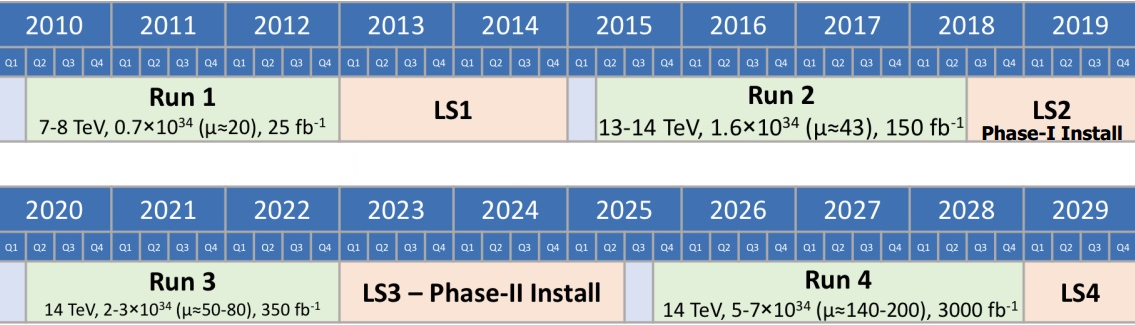
\includegraphics[width=0.8\textwidth]{Figures/Intro/LHCrunplan_modif.png}
\end{center}

\begin{small}
\begin{maliste}
\item Activités sur \ATLAS{} entre 2008 et 2015
\vspace*{0.1cm}
\begin{itemize}
\item 2008 - 2009 puis 2011 $\rightarrow$ 2015 : recherche de nouvelle physique
\vspace*{0.05cm}
\item 2009 $\rightarrow$ 2012 : calibration des jets
\vspace*{0.05cm}
\item Interpr\'etation statistique
\end{itemize}
\vspace*{0.1cm}
\item Co-encadrement de 2 doctorants
\end{maliste}
\end{small}

\begin{center}
\includegraphics[width=0.38\textwidth]{Figures/Intro/sumLumiByWeek.png}
\includegraphics[width=0.38\textwidth]{Figures/Intro/intlumivstime2012DQ.png}
\end{center}
\end{frame}

\begin{frame}
\frametitle{D\'etecteur ATLAS}

\begin{center}
\vspace*{-0.3cm}
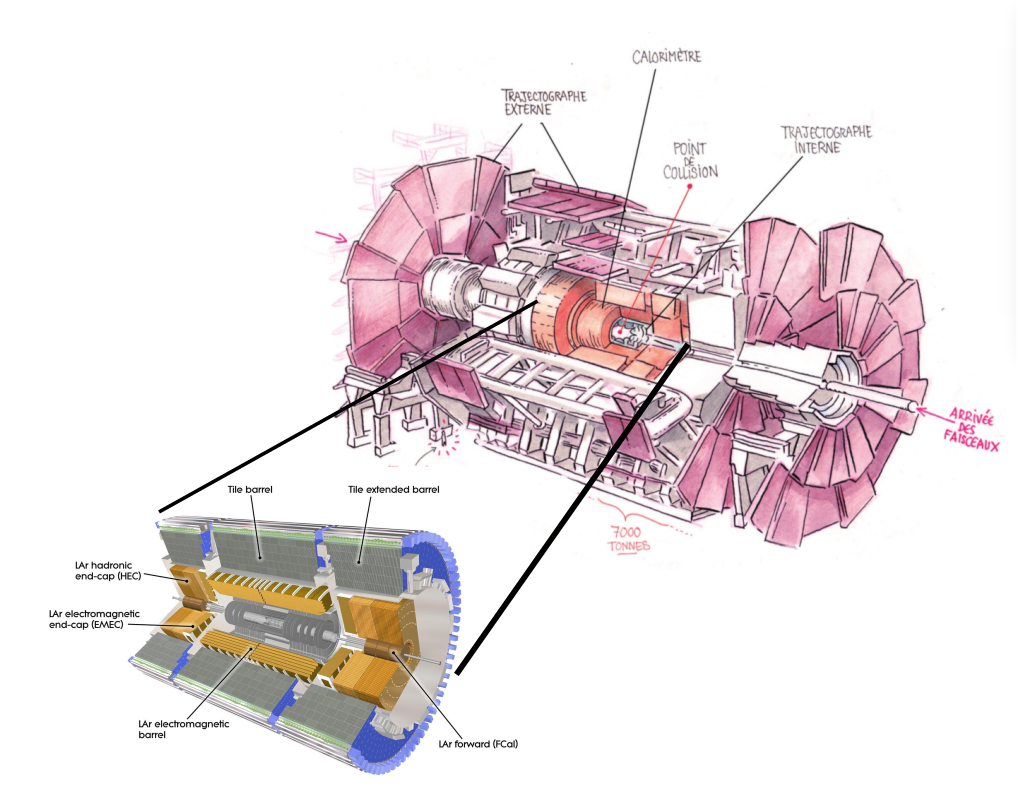
\includegraphics[width=1\textwidth]{Figures/Intro/ATLAS_full.png}
\end{center}

\end{frame}



%\begin{comment}
\section{Calibration des jets}
\begin{comment}
\begin{frame}[plain]
\begin{center}
\textbf{\Large Calibration des jets}
\end{center}
\end{frame}
\end{comment}

\begin{frame}
\frametitle{Calibration des jets}
\begin{columns}
\begin{column}{0.7\textwidth}
\begin{maliste}
%\item Premières données de 2010 : \textcolor{red}{XX~fb$^{-1}$}
\item Production massive de jets au LHC
\vspace*{0.2cm}
\item Acc\`es aux particules instables : top, W, Higgs, etc.
\vspace*{0.2cm}
\item Nécessité d'une calibration : non-compensation, matériaux morts, out-of-cone, ...
\vspace*{0.2cm}
\item Objet de référence : jet de particules 
\begin{itemize}
%\item Algorithme : \antikt
\item Input : particules stables après hadronisation (sauf muons et neutrinos)
\item \'Energie : \Etruth
\end{itemize}
\end{maliste}
\end{column}
\begin{column}{0.35\textwidth}
\includegraphics[width=.9\textwidth]{Figures/JES/jetAtVariousLevelIllustration.png}
\end{column}
\end{columns}
\begin{center}
\begin{minipage}{4cm}
\begin{varblock}[5cm]{}
\begin{normalsize}
\textcolor{blue}{Objectifs : $R=\left<E/\Etruth\right>\simeq 1$}
\begin{itemize}
\item \textcolor{blue}{Petite incertitude sur $R$}
\item \textcolor{blue}{Bonne résolution en énergie}
\end{itemize}
\end{normalsize}
\end{varblock}
\end{minipage}
\end{center}
\end{frame}

\begin{frame}
\frametitle{Les 4 calibrations dans ATLAS au d\'ebut du run 1}

\vspace*{-0.3cm}
\begin{columns}
\begin{column}{0.5\textwidth}
\begin{block}{EM+JES}
\begin{itemize}
%\item Calibration la plus simple
\item Apr\`es calibration : $R(p_T,\eta)=1$
\item Constantes d\'eriv\'ees au tout d\'ebut du run 1 (stage M2 J. Demaizi\`ere)
\begin{center}
\includegraphics[scale=0.2]{Figures/JES/fig_09_responseEMscaleVsEta.pdf}
\end{center}
\end{itemize}
\end{block}
\end{column}
\pause
\begin{column}{0.55\textwidth}
{
\setbeamercolor{block title}{use=structure,fg=white,bg=green!20!black}
\setbeamercolor{block body}{use=structure,fg=black,bg=green!10!white}
\begin{block}{GCW+JES {\small (``Global Cell Weighting'')}}
\begin{itemize}
\item Principe : calibration bas\'ee sur densit\'e d'\'energie des cellules $E/V$
\item Minimisation \\
\begin{scriptsize}
\[\chi^2=\sum\limits_\text{jets}\left(E^{GCW}/E^{truth}-1\right)^2\]
\end{scriptsize}
\\
avec \\
\begin{scriptsize}
\[E^{GCW}=\sum\limits_{i: \text{cellules}} w_i\left(E_i/V_i\right)E_i\]
\end{scriptsize}
\item JES pour restaurer $R(p_T,\eta)=1$
\end{itemize}
\end{block}
}
\end{column}
\end{columns}
\pause
\begin{columns}
\begin{column}{0.65\textwidth}
{
\setbeamercolor{block title}{use=structure,fg=white,bg=magenta!60!black}
\setbeamercolor{block body}{use=structure,fg=black,bg=magenta!10!white}
\begin{block}{LCW+JES {\small (``Local Cell Weighting'')}}
\begin{columns}
\begin{column}{0.4\textwidth}
\vspace*{-0.5cm}
\begin{center}
\includegraphics[scale=0.2]{Figures/JES/topoclusterillustration.png}
\end{center}
\end{column}
\hspace{-1cm}
\begin{column}{0.75\textwidth}
\begin{itemize}
\item Calibration clusters\\
$\rightarrow$ non-compensation, out-of-cluster, mat\'eriaux morts
\item JES pour restaurer $R(p_T,\eta)=1$\\
$\rightarrow$ out-of-cone, inefficacit\'es 
\end{itemize}
\end{column}
\end{columns}
\end{block}
}
\end{column}
\pause
\begin{column}{0.35\textwidth}
{
\setbeamercolor{block title}{use=structure,fg=white,bg=purple!75!black}
\setbeamercolor{block body}{use=structure,fg=black,bg=purple!20!white}
\begin{block}{GS {\small (``Global Sequential'')}}
\begin{itemize}
\item EM+JES puis calibration globale
\item cf pages suivantes
\end{itemize}
\end{block}
}
\end{column}
\end{columns}

%\begin{maliste}
%\item 4 calibrations existaient en 2009 :
%\begin{itemize}
%\item EM+JES (prendre du temps pour l'expliquer -> notamment bien dire qu'apre%s reponse = 1, sinon on ne comprendra pas les plots GS)
%\item Global Cell Weighting : GCW
%\item Local Cell Weighting : LCW
%\item Global Sequential Calibration : GS
%\end{itemize}
%\end{maliste}
\end{frame}

\begin{frame}
\frametitle{Calibration Globale S\'equentielle (GS) : principe}
\begin{columns}
\begin{column}{0.75\textwidth}
\begin{small}
\begin{maliste}
\item \'Equipe : Reina Camacho, David Lopez-Mateos, Ariel Schwartzman
\vspace*{0.2cm}
\item \textcolor{magenta}{Eur.Phys.J. C73 (2013) 2304}\\
\textcolor{magenta}{Eur.Phys.J. C73 (2013) 2306}
\vspace*{0.2cm}
\item \EMJES{} supprime dépendance en $\eta$ et $\pt$
\begin{center}
$\rightarrow$ subsiste d'autres dépendances\\
$\rightarrow$ GS les supprime
\end{center}
\item Apr\`es GS : $R(p_T,\eta,x)=1$ ($x$ : variable corr\'el\'ee \`a la r\'eponse)
\vspace*{0.2cm}
\item Int\'er\^et principal : meilleure r\'esolution
\end{maliste}
\end{small}
\end{column}
\begin{column}{0.3\textwidth}
\begin{center}
\hspace*{-0.5cm}
\includegraphics[scale=0.185]{Figures/JES/responseDependenceWidthIllustration.png}
\end{center}
\end{column}
\end{columns}
%\[
%\pt^\GS=\left(\prod\limits_{n=1}^{N}C_n(x_n)\right)\times \pt^\EMJES
%\]
\end{frame}

\begin{frame}
\frametitle{Calibration GS : propri\'et\'es utilis\'ees}
\begin{columns}
\begin{column}{0.6\textwidth}
\begin{center}
\hspace*{-2cm}
\includegraphics[width=.9\textwidth]{Figures/JES/EventDisplayJet_modified.png}
\hspace*{-1.2cm}
\includegraphics[width=.62\textwidth]{Figures/JES/c_fracs_vs_pt.png}
\end{center}
\end{column}
\begin{column}{0.55\textwidth}
\begin{maliste}
\item Propriétés :
\begin{itemize}
\item longitudinales : $f_{\rm layer}=\frac{E_\EM^{\rm layer}}{E_\EM^{\rm jet}}$
\item transversales : $\width$
\end{itemize}
\vspace*{0.3cm}
\item Plusieurs propri\'et\'es utilis\'ees de mani\`ere s\'equentielle
\[
\pt^\GS=\left(\prod\limits_{n=1}^{N}C_n(x_n)\right)\times \pt^\EMJES
\]
%avant de pouvoir l'appliquer aux autres types d'evts il faut verifier que la calibration est exportable.
\end{maliste}
\end{column}
\end{columns}

%\begin{maliste}
%\item Choix des propri\'et\'es empirique
%\vspace*{0.2cm}
%\item Calibration d\'eriv\'ee pour $0<|\eta|<4,5$ et $p_T<800~$GeV
%$45\times 20 \times 25$ bins en $(\eta,x,p_T)$
%\end{maliste}
\end{frame}

\begin{comment}
\begin{frame}
\frametitle{Calibration GS : effet sur la r\'eponse}
\includegraphics[width=0.5\textwidth]{Figures/JES/fig_46b.pdf}
\includegraphics[width=0.5\textwidth]{Figures/JES/fig_46a.pdf}

\vspace*{0.2cm}
\begin{maliste}
\item Quel effet sur la r\'esolution ?\\
\vspace*{0.1cm}
\item Calibration d\'eriv\'ee sur \'echantillon simul\'e multijets\\
\vspace*{0.1cm}
\begin{center}
\textcolor{magenta}{$\rightarrow$ Peut-on l'appliquer \`a d'autres \'echantillons simul\'es et aux donn\'ees ?}
\end{center}
\end{maliste}
\end{frame}
\end{comment}

\begin{frame}
\frametitle{Calibration GS : performances}
\vspace*{-0.8cm}
\begin{maliste}
\item R\'esolution sur simulation et donn\'ees
%\begin{center}
\hspace*{-1cm}
\includegraphics[width=.48\textwidth]{Figures/JES/GSCPerfResolOnMC.png}
\includegraphics[width=.54\textwidth]{Figures/JES/fig_13a.jpg}
%\end{center}
\begin{center}
$\rightarrow$ Am\'elioration de 20\% \`a 30\% pour $p_T>150$ GeV 
\end{center}

\hspace*{7cm}
\includegraphics[width=.35\textwidth]{Figures/JES/fig_78a.jpg}
\vspace*{-3.5cm}
\item D\'ependance avec la saveur du jet\\
\vspace*{0.1cm}
$\rightarrow$ r\'eponse diff\'erente pour quarks et gluons\\
\vspace*{0.1cm}
$\rightarrow$ r\'eponse moyenne d\'epend de la composition\\
en saveur
\end{maliste}
\end{frame}

\begin{frame}
\frametitle{Calibration GS : validation sur les données}
\vspace*{-0.2cm}
\begin{maliste}
\item Calibration GS peut-\^etre d\'eriv\'ee sur les donn\'ees r\'eelles

\vspace*{0.3cm}
\begin{columns}
\begin{column}{0.5\textwidth}
\includegraphics[width=1\textwidth]{Figures/JES/DijetsEventDisplay.png}
\end{column}
\begin{column}{0.5\textwidth}
\[A(x)=2\frac{p_T^\text{probe}(x)-p_T^\text{ref}}{p_T^\text{probe}(x)+p_T^\text{ref}}\]
\vspace*{-0.1cm}
\[
\hspace*{1cm}
\Rightarrow
\left<R(x)\right>\simeq\frac{2+\left<A(x)\right>}{2-\left<A(x)\right)}
\]
\end{column}
\end{columns}
\vspace*{0.2cm}
\item M\'ethode valid\'ee sur simulation puis appliqu\'ee aux donn\'ees
\vspace*{-0.1cm}
\end{maliste}
\begin{center}
%\includegraphics[width=.4\textwidth]{Figures/JES/fig_47c.pdf}
\includegraphics[width=.4\textwidth]{Figures/JES/fig_49c.pdf}
\end{center}
\vspace*{-0.35cm}
\begin{center}
\textcolor{magenta}{$\rightarrow$ calibration GS valid\'ee avec 38~pb$^{-1}$ !}
\end{center}
\end{frame}

\begin{frame}
\frametitle{Calibration GS : diff\'erences donn\'ees/simulation}

\begin{maliste}
\item Erreurs sur propri\'et\'es $\Rightarrow$ Incertitude sur r\'eponse moyenne
\includegraphics[width=.37\textwidth]{Figures/JES/fig_50c.pdf}
\quad
\includegraphics[width=.37\textwidth]{Figures/JES/fig_50d.pdf}
\end{maliste}

\vspace*{-0.5cm}
\begin{columns}
\begin{column}{0.3\textwidth}
\vspace{-0.5cm}
\begin{center}
%\includegraphics[width=0.7\textwidth]{Figures/JES/fig_51c.pdf}
\includegraphics[width=1.2\textwidth]{Figures/JES/fig_51c.pdf}
\end{center}
\end{column}
\begin{column}{0.6\textwidth}
\begin{maliste}
\item[$\rightarrow$] Incertitude estim\'ee sur evts multi-jets, $\gamma$+jets, sans et avec pile-up
\vspace*{0.3cm}
\item[$\rightarrow$] R\'esultat : incertitude syst. $\simeq 1$\%
\vspace*{0.3cm}
\item[$\Rightarrow$] GS induit une d\'egradation minime de l'\'echelle en \'energie
\end{maliste}
\end{column}
\end{columns}
\end{frame}

\begin{frame}
\frametitle{Ce qu'il reste}
\begin{maliste}
%\item Calibration des jets sur les premi\`eres donn\'ees : EM+JES et GS
%\vspace*{0.5cm}
\item Nous avons montr\'e que GS est une calibration : 
\begin{itemize}
\item relativement simple \`a mettre en \oe uvre
\item performante 
\item facile à valider sur les donn\'ees
\end{itemize}
%\vspace*{0.2cm}
\hspace*{7cm}
\includegraphics[width=0.33\textwidth]{Figures/JES/HbbPlotMbbVsMbbtrue.png}
%\includegraphics[width=0.4\textwidth]{Figures/JES/MbbPlotPublic.png}
\vspace*{-3.cm}
%\item Notre travail = preuve de concept
\vspace*{0.5cm}
\item GS utilis\'ee pour la premi\`ere fois pour \\la recherche $H\rightarrow b\bar{b}$
\vspace*{0.5cm}
\item \'Etat actuel dans ATLAS :
\vspace*{0.3cm}
\begin{itemize}
\item GS utilis\'ee en combinaison avec LCW
\hspace*{-0.8cm}
\includegraphics[width=1\textwidth]{Figures/JES/CurrentATLASJetCalib_modified.png}
\end{itemize}
\end{maliste}
\end{frame}



\section{Recherche de nouvelle physique}

\begin{comment}
\begin{frame}[plain]
\begin{center}
\textbf{\Large Recherche d'événements avec 4 quarks top}
\end{center}
\end{frame}
\end{comment}


\begin{frame}
\frametitle{Quark top et nouvelle physique}

\begin{columns}
\begin{column}{0.12\textwidth}
\hspace*{-1cm}
\includegraphics[width=2.2\textwidth]{Figures/FourTops/TopDecay.png}
\end{column}
\begin{column}{0.78\textwidth}
\begin{varblock}[8cm]{Quark top}
\begin{maliste}
\item[$\rightarrow$] Masse = $173,34\pm 0,76$~GeV
\item[$\rightarrow$] Fen\^etre sur EWSB
%\item Désintégration précède hadronisation
\item[$\rightarrow$] Désintégration ``facilement'' observable
\item[$\rightarrow$] Modes de production : paire, c\'elibataire
\end{maliste}
\end{varblock}
\end{column}
\hspace*{-1cm}
\begin{column}{0.1\textwidth}
\includegraphics[width=1.6\textwidth]{Figures/FourTops/feyndiag_ttbar.png}\\
\includegraphics[width=1.5\textwidth]{Figures/FourTops/feyndiag_singletop_tchannel.png}
\end{column}
\end{columns}

\begin{center}
\hspace*{-1cm}
\includegraphics[width=0.3\textwidth]{Figures/FourTops/fig_resonancettbar.png}
\hspace*{-0.2cm}
\includegraphics[width=0.35\textwidth]{Figures/FourTops/fig_monotop.png}%\\
%\vspace*{-0.5cm}
%\hspace*{1cm}
\hspace*{-0.15cm}
\includegraphics[width=0.23\textwidth]{Figures/FourTops/fig_Wprime.png}
\hspace*{-0.1cm}
\includegraphics[width=0.3\textwidth]{Figures/FourTops/singletop_summaryplot.png}
\end{center}

\begin{maliste}
%\item Panorama des searches dans secteur du top (avec dimension historique) : top pair, single top (mettre plot ou valeurs xsec ?)
\item[$\rightarrow$] Nouveau mode de production : \'evénements 4 tops 
\begin{itemize}
\item Compl\'ementaire des autres modes de production
%Dire quelque chose sur complémentarité entre 4tops et les autres (single 
%top et top pair) : ex : 4tops par 2HDM peut apporter quelque chose par rapport 
%a ttbar car dans cas ttbar il y a interference importante qui peut rendre 
%analyse difficile
%\item Cet article peut etre interessant (pour voir mesures dans secteur du top qui sont utilisees pour contraindre les operateurs de nouvelle physique et le resultat de ces contraintes) : http://arxiv.org/pdf/1506.08845v1.pdf
\item LHC = premier labo permettant recherche 4 tops
%\item Pas si r\'ecents que cela ...
\end{itemize}
\end{maliste}
\end{frame}

\begin{frame}
\frametitle{}
\begin{center}
\vspace*{-0.7cm}
\includegraphics[width=1\textwidth]{Figures/FourTops/TheFourTopsMusic.jpg}
\end{center}
\end{frame}

\begin{comment}
\begin{frame}
\frametitle{Historique}

\begin{figure}[!htb]
\begin{center}
\vspace*{-0.8cm}
%\vspace*{-1cm}
\hspace*{-0.5cm}
\includegraphics<1>[width=1.13\textwidth]{friseChrono4tops_1.pdf}
\vspace*{-5cm}
\hspace*{1cm}
\includegraphics<1>[width=0.4\textwidth]{Figures/FourTops/4topCalculationsFromBarger91.png}
\includegraphics<2>[width=1.13\textwidth]{friseChrono4tops_2.pdf}
\includegraphics<3>[width=1.13\textwidth]{friseChrono4tops_3.pdf}
\end{center}
\end{figure}
\end{frame}
\end{comment}

\begin{frame}
\frametitle{Historique}

\begin{figure}[!htb]
\begin{center}
\vspace*{-0.8cm}
%\vspace*{-1cm}
\hspace*{-0.5cm}
\includegraphics[width=1.13\textwidth]{friseChrono4tops_1.pdf}
\vspace*{-5cm}
\hspace*{1cm}
\includegraphics[width=0.4\textwidth]{Figures/FourTops/4topCalculationsFromBarger91.png}
\end{center}
\end{figure}
\end{frame}

\begin{frame}
\frametitle{Historique}
\begin{figure}[!htb]
\begin{center}
\vspace*{-0.5cm}
%\vspace*{-1cm}
\hspace*{-0.5cm}
\includegraphics<1>[width=1.13\textwidth]{friseChrono4tops_2test.pdf}
\includegraphics<2>[width=1.13\textwidth]{friseChrono4tops_3testarticleref.pdf}
\end{center}
\end{figure}
\end{frame}

\begin{frame}
\frametitle{Stratégie de recherche}
\begin{small}
\begin{maliste}
\item \'Equipe : David Calvet, Daniela Paredes, Lo\"ic Valery, Dorian Simon, ...
%\vspace*{0.1cm}
%\item \textcolor{magenta}{JHEP 10 (2015) 150}
\vspace*{0.1cm}
\item Processus 4 tops considérés : \textcolor{blue}{non-r\'esonant, r\'esonant, mod\`ele standard}
\end{maliste}
\end{small}

\begin{varblock}[11cm]{Contexte}
\begin{columns}
\begin{column}{0.6\textwidth}
\begin{itemize}
\item Groupe d'analyse : ``same-sign dilepton''
\item Signaux considérés : 
\begin{itemize}
\item[$\rightarrow$] sgluon, VLQ, tt, b', T5/3, ...
\end{itemize}
\end{itemize}
\end{column}
\begin{column}{0.4\textwidth}
%\hspace*{-1.5cm}
%\includegraphics[width=0.6\textwidth]{Figures/FourTops/4topsSMfeynSnapshot.png}
\includegraphics[width=0.65\textwidth]{Figures/FourTops/VLQ_feynDiag.png}

\end{column}
\end{columns}
\end{varblock}

\begin{varblock}[11cm]{Signature}
\begin{columns}
\begin{column}{0.5\textwidth}
\hspace*{0.8cm}
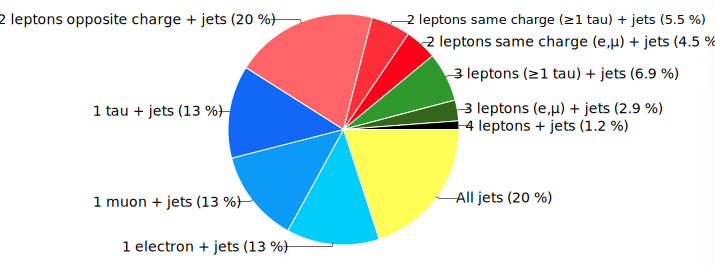
\includegraphics[width=1.2\textwidth]{Figures/FourTops/pie_chart_testinkscape.png}
\end{column}
\hspace*{1.5cm}
\begin{column}{0.5\textwidth}
\begin{maliste}
\item 2 leptons de même charge \\
ou 3 leptons
\item grand nombre de $b$
\item grande $\ETmiss$ 
\item grand $H_T$ 
\end{maliste}
\end{column}
\end{columns}
\end{varblock}
\end{frame}

\begin{frame}
\frametitle{Productions MS et non-résonante}

\begin{maliste}
\item \textcolor{blue}{Production modèle standard}
\begin{columns}
\begin{column}{0.4\textwidth}
\begin{figure}
\begin{center}
\vspace*{-0.5cm}
\hspace*{2cm}
\scalebox{0.65}{
\begin{fmffile}{fgraph-4topsSM}
\begin{fmfgraph*}(110,60)
\fmfleftn{i}{2}\fmfrightn{o}{4}
\fmfset{curly_len}{2mm}
\fmflabel{$g$}{i1}
\fmflabel{$g$}{i2}
\fmflabel{$t$}{o1}
\fmflabel{$\overline{t}$}{o2}
\fmflabel{$t$}{o3}
\fmflabel{$\overline{t}$}{o4}
\fmf{gluon}{i1,v1}
\fmf{fermion}{v1,o1}
\fmf{fermion}{v2,v1}
\fmf{fermion}{o2,v4}
\fmf{gluon}{i2,v3}
\fmf{fermion}{o4,v3}
\fmf{fermion}{v3,v2}
\fmf{fermion}{v4,o3}
\fmf{gluon}{v2,v4}
\fmffixedx{40}{i1,v1}
\fmffixedx{40}{i2,v3}
\end{fmfgraph*}
\end{fmffile}
}
\end{center}
\end{figure}
%\hspace*{0.5cm}
\vspace*{0.1cm}
%\begin{center}
\[\qquad \qquad \quad \quad\sigma\simeq 1~\text{fb \`a }\sqrt{s}=8~\text{TeV}\]
%\end{center}
\end{column}
\begin{column}{0.6\textwidth}
\begin{center}
\vspace*{-0.8cm}
\hspace*{1cm}
\includegraphics[width=0.8\textwidth]{Figures/FourTops/1234topsSMxsec.png}
\end{center}
\end{column}
\end{columns}
\pause
%\vspace*{0.5cm}
\item \textcolor{blue}{Production non-résonante : interaction contact à 4 tops}
\end{maliste}
\begin{columns}
\hspace*{1cm}
\begin{column}{0.6\textwidth}
\[{\cal L} = {\cal L}_\text{SM}+\frac{C}{\Lambda^2}\left(\bar{t}_R\gamma_{ \mu} t_R\right)\left(\bar{t}_R\gamma^{\mu} t_R\right)\]
\begin{itemize}
%\item Interaction contact à 4 tops
%\[{\cal L} = {\cal L}_\text{SM}+\frac{C}{\Lambda^2}\left(\bar{t}_R\gamma_{ \mu} t_R\right)\left(\bar{t}_R\gamma^{\mu} t_R\right)\]
\item Physique BSM avec nouveau vecteur\\
$\rightarrow$ masse $M$\\
$\rightarrow$ limite valable si $M\gtrsim 2$~TeV
\item Pas de contraintes sur $\frac{C}{\Lambda^2}$
\end{itemize}
\end{column}
%\vspace*{0.5cm}
\hspace*{-1cm}
\begin{column}{0.4\textwidth}
\begin{figure}[!htb]
\begin{center}
\scalebox{0.6}{
\begin{fmffile}{fgraph-ContactGluFu1}
\begin{fmfgraph*}(110,60)
\fmfleftn{i}{2}\fmfrightn{o}{4}
\fmfset{curly_len}{2mm}
\fmflabel{$g$}{i1}
\fmflabel{$g$}{i2}
\fmflabel{$t$}{o1}
\fmflabel{$\overline{t}$}{o2}
\fmflabel{$t$}{o3}
\fmflabel{$\overline{t}$}{o4}
\fmf{gluon}{i1,v1}
\fmf{gluon}{i2,v1}
\fmf{gluon,label=$g$}{v1,v2}
\fmf{fermion}{v2,o1}
\fmf{fermion}{v3,v2}
\fmf{fermion}{o2,v3}
\fmf{fermion}{v3,o3}
\fmf{fermion}{o4,v3}
\fmffixedx{20}{i1,v1}
\fmffixedx{20}{i2,v1}
\fmffixed{(25,0)}{v1,v2}
\fmffixed{(25,10)}{v2,v3}
\fmfblob{.07w}{v3}
\end{fmfgraph*} \hspace*{0.8cm}
\end{fmffile}
}
\end{center}
\end{figure}
\begin{figure}[!htb]
\begin{center}
\scalebox{0.6}{
\begin{fmffile}{fgraph-ContactGluFu2}
\begin{fmfgraph*}(110,60)
\fmfleftn{i}{2}\fmfrightn{o}{4}
\fmfset{curly_len}{2mm}
\fmflabel{$g$}{i1}
\fmflabel{$g$}{i2}
\fmflabel{$t$}{o1}
\fmflabel{$\overline{t}$}{o2}
\fmflabel{$t$}{o3}
\fmflabel{$\overline{t}$}{o4}
\fmf{gluon}{i1,v1}
\fmf{fermion}{v1,o1}
\fmf{fermion}{v2,v1}
\fmf{fermion}{o2,v2}
\fmf{gluon}{i2,v3}
\fmf{fermion}{o4,v3}
\fmf{fermion}{v3,v2}
\fmf{fermion}{v2,o3}
\fmffixedx{40}{i1,v1}
\fmffixedx{40}{i2,v3}
\fmfblob{.07w}{v2}
\end{fmfgraph*}
\end{fmffile}
}
\end{center}
\end{figure}
\end{column}
\end{columns}

\end{frame}

\begin{frame}
\frametitle{Production effective : interaction de contact}
\begin{center}
Exemples de modèles conduisant à une interaction de contact
\end{center}
\begin{columns}
\begin{column}{0.5\textwidth}
\begin{block}{\center Top composite (arXiv:0712.3057,1010.6340,...)}
\vspace*{0.2cm}
\begin{figure}
\begin{center}
\scalebox{0.65}{
\begin{fmffile}{fgraph-TopComposite}
\begin{fmfgraph*}(110,60)
\fmfleftn{i}{2}\fmfrightn{o}{4}
\fmfset{curly_len}{2mm}
\fmflabel{$g$}{i1}
\fmflabel{$g$}{i2}
\fmflabel{$t$}{o1}
\fmflabel{$\overline{t}$}{o2}
\fmflabel{$t$}{o3}
\fmflabel{$\overline{t}$}{o4}
\fmf{gluon}{i1,v1}
\fmf{fermion}{v1,o1}
\fmf{fermion}{v2,v1}
\fmf{fermion}{o2,v4}
\fmf{gluon}{i2,v3}
\fmf{fermion}{o4,v3}
\fmf{fermion}{v3,v2}
\fmf{fermion}{v4,o3}
\fmf{photon,label=$\rho$}{v2,v4}
\fmffixedx{40}{i1,v1}
\fmffixedx{40}{i2,v3}
\end{fmfgraph*}
\end{fmffile}
}
\end{center}
\end{figure}
\vspace*{-0.3cm}
\begin{figure}[!htb]
\begin{center}
%\includegraphics[width=0.75\textwidth]{Figures/FourTops/TopCompositeXsecJingShuEtAl.png}
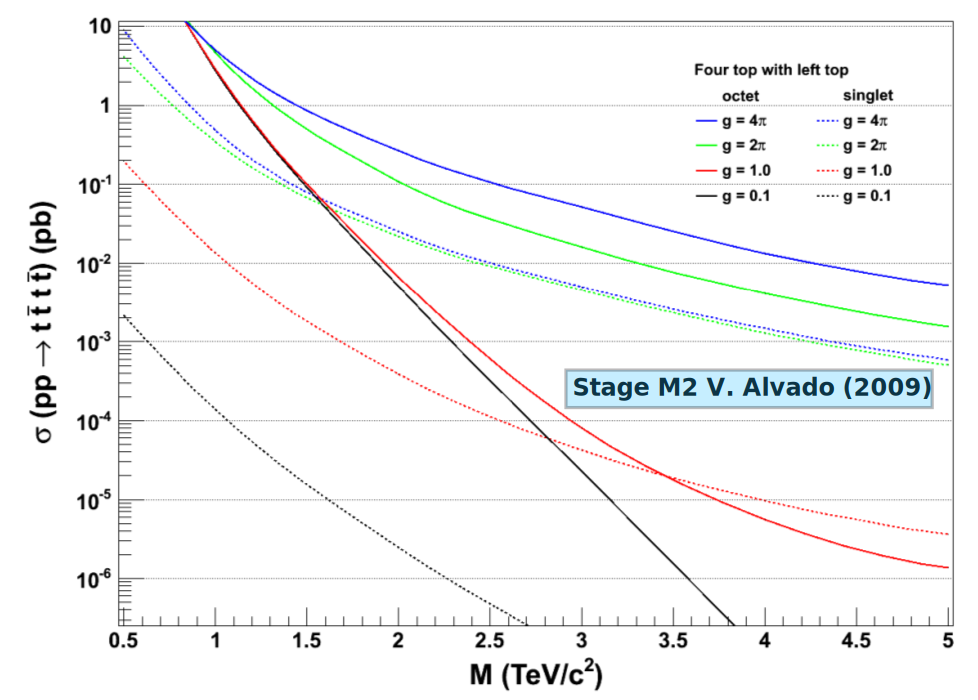
\includegraphics[width=0.95\textwidth]{Figures/FourTops/PlotVincentAlvado.png}
\put(-40,35){\tiny{$\sqrt{s}=14~$TeV}}
\end{center}
\end{figure}

\end{block}
\pause
\end{column}
\begin{column}{0.55\textwidth}
\begin{block}{\center RS modifié $t\bar{t} g_{KK}$ (arXiv:0710.2234)}
\begin{itemize}
\item Champs standards dans bulk
\item Higgs sur TeV brane
\item Couplage fort entre $g_{KK}$ et $t_R$
%\item Couplage $ggg_{KK}$ supprimé (profiles $\perp$)
%\item Processus favorisé : $gg(q\bar{q})\rightarrow t_R \bar{t}_R g_{KK}$
\end{itemize}

\begin{figure}
\begin{center}
\scalebox{0.65}{
\begin{fmffile}{fgraph-ttbargKKproduction}
\begin{fmfgraph*}(110,60)
\fmfleftn{i}{2}\fmfrightn{o}{3}
\fmfset{curly_len}{2mm}
\fmflabel{$g$}{i1}
\fmflabel{$g$}{i2}
\fmflabel{$t$}{o1}
\fmflabel{$\overline{t}$}{o2}
\fmflabel{$g_{KK}$}{o3}
\fmf{gluon}{i1,v1}
\fmf{gluon}{v1,i2}
\fmf{gluon,label=$g$}{v1,v2}
\fmf{fermion}{v2,o1}
\fmf{fermion}{v3,v2}
\fmf{fermion}{o2,v3}
\fmf{gluon}{v3,o3}
\fmffixedx{25}{i1,v1}
\fmffixedx{25}{i2,v1}
\fmffixed{(20,0)}{v1,v2}
%\fmffixed{(30,10)}{v2,v3}
\end{fmfgraph*} 
\end{fmffile}
}
\end{center}
\end{figure}
\vspace*{0.2cm}

\end{block}
\pause
\begin{block}{Z' \english{top-philic} (arXiv:0912.0004)}
\begin{itemize}
\item $SU(3)_C\times SU(2)_L\times U(1)_Y \times U(1)'$\\
$\rightarrow Z'$ et $\nu'$ (candidat DM)
\item Processus favorisé : $gg(q\bar{q})\rightarrow t_R \bar{t}_R Z'$
%\item Couplage fort $Z'tt_R$
\end{itemize}
\end{block}
\end{column}
\end{columns}
\end{frame}

\begin{frame}
\frametitle{Production résonante : modèle 2UED/RPP}

\begin{textblock*}{5cm}(.95\textwidth,0.4cm)%
  \scriptsize{ 
    \textcolor{white}{arXiv:0907.4993}\\
    \textcolor{white}{arXiv:1104.3800}\\
    \textcolor{white}{arXiv:1107.4616}\\
    arXiv:1209.6556\\
    arXiv:1210.0384\\
    arXiv:1302.4750
  }
\end{textblock*}

\MyTextNoTilt{\'Etage : $(k,l)$}
\begin{maliste}
\item Extension ``simple'' du modèle standard :
\begin{itemize}
\item 2 dimensions supplémentaires universelles
\item Compactification : Real Projective Plane (RPP)
\end{itemize} 
\vspace*{0.1cm}
\item Intérêt : candidat matière noire (photon $A^{\left(1,0\right)}$)
\end{maliste}
\begin{columns}
\begin{column}{0.5\textwidth}
%\vspace*{0.1cm}
\begin{figure}
\includegraphics[width=0.95\textwidth]{Figures/FourTops/cosmoConstraints2UEDRPP_symmetric.png}
\put(-95,88){\scriptsize{JHEP, 1301 : 147, 2013}}
\put(-40,70){\scriptsize{$R_4= R_5$}}
\end{figure}
\vspace*{-1.28cm}
\begin{figure}
\includegraphics[width=0.98\textwidth]{Figures/FourTops/cosmoConstraints2UEDRPP.png}
\put(-40,25){\scriptsize{$R_4\neq R_5$}}
\end{figure}
\end{column}
\hspace*{-0.3cm}
\begin{column}{0.55\textwidth}
\begin{block}{Paramètres}
\begin{maliste}
\item Rayons : $R_4$, $R_5$
\[
\begin{pmatrix}
R_4 \\
R_5
\end{pmatrix}
\Rightarrow
\begin{pmatrix}
\xi=\frac{R_4}{R_5} \\
m_\text{KK}=\frac{1}{R_4}
\end{pmatrix}
\]
\vspace*{0.1cm}
\item Cut-off : $\Lambda$
\item Rapport embranchement : $A^{(1,1)}\rightarrow t\bar{t}$
\end{maliste}
\end{block}
\begin{block}{Contraintes cosmologiques}
\begin{maliste}
\item $\xi=1$ défavorisé
\item $m_\text{KK}\in\left[700;1000\right]$~GeV 
\end{maliste}
\end{block}
\end{column}
\end{columns}
\end{frame}

\begin{frame}
\frametitle{2UED/RPP : phénoménologie au LHC}
\begin{maliste}
\item Phénoménologie riche : contributions étages $(1,0)$, $(1,1)$ et $(2,0)$
\item Contraintes à partir des étages $(1,0)$, $(2,0)$ : $m_\text{KK}\gtrsim 600~$GeV %(arXiv:1209.6556,arXiv:1302.4750)
\item \textcolor{magenta}{\'Etages $(1,1)$ et $(2,0)$ : événements 4 tops}

\vspace*{0.3cm}
\begin{figure}
\begin{center}
\scalebox{0.55}{
\begin{fmffile}{fgraph-2UEDRPP}
\unitlength = 0.45mm

\begin{fmfgraph*}(160,90)

%\fmfpen{thick}                                                                                       
\fmfleft{i2,i1}
\fmfright{t1,t2,t3,t4}
\fmftop{i1,p1,p2,a5,a6,a7,t4}
\fmfbottom{i2,p3,a1,a2,a3,a4,t1}
\fmfset{curly_len}{2mm}
\fmf{fermion,tension=1}{i1,v1}
\fmf{fermion,tension=.2}{v8,a5}
\fmf{fermion,tension=.2}{a6,v9}
\fmf{fermion,tension=.2}{v10,a7}
\fmf{fermion,tension=.5}{t3,v11,t4}
\fmf{fermion,tension=.2}{a1,v3}
\fmf{fermion,tension=.2}{v4,a2}
\fmf{fermion,tension=.2}{a3,v5}
\fmf{fermion,tension=.2}{v6,a4}
\fmf{fermion,tension=.5}{t1,v7,t2}

\fmf{gluon,tension=1}{i2,v2}


\fmf{gluon,label=${\scriptstyle g}^{\scriptscriptstyle (1,,1)}\;\;$}{v1,v2}
\fmf{gluon,tension=1.2}{v2,v3}
\put(37,33){${\scriptstyle g}^{\scriptscriptstyle (1,1)}$}

\fmf{boson,label=${\scriptstyle W}^{\scriptscriptstyle +(1,,1)}$}{v8,v9}
\fmf{boson,label=${\scriptstyle Z}^{\scriptscriptstyle (1,,1)}$,l.s=left}{v4,v5}
\fmf{boson,tension=0.6}{v6,v7}
\put(120,20){${\scriptstyle A}^{\scriptscriptstyle (1,1)}$}

\fmf{boson,tension=0.6}{v10,v11}
\put(115,62){${\scriptstyle A}^{\scriptscriptstyle (1,1)}$}

\fmf{fermion,tension=1.2,label=${\scriptstyle u_L}^{\scriptscriptstyle (1,,1)}$}{v1,v8}
\fmf{fermion,label=${\scriptstyle \nu_\tau}^{\scriptscriptstyle (1,,1)}$,l.s=right}{v9,v10}
\fmf{fermion,label=$\;\;{\scriptstyle c_{L}}^{\scriptscriptstyle (1,,1)}$,l.s=left}{v3,v4}
\fmf{fermion,label=$\;\;{\scriptstyle \mu}^{\scriptscriptstyle -(1,,1)}\;\;$,l.s=left}{v5,v6}
\fmfblob{.04w}{v11}
\fmfblob{.04w}{v7}
%\fmfv{decor.shape=circle,decor.filled=full,decor.size=10}{v11}                                       
%\fmfv{decor.shape=circle,decor.filled=full,decor.size=10}{v7}   

\fmflabel{$u$}{i1}
\fmflabel{$g$}{i2}
\fmflabel{\textcolor{blue}{$\bar{c}$}}{a1}
\fmflabel{\textcolor{blue}{$c$}}{a2}
\fmflabel{\textcolor{blue}{$\mu^+$}}{a3}
\fmflabel{\textcolor{blue}{$\mu^{-}$}}{a4}
\fmflabel{\textcolor{blue}{$d$}}{a5}
\fmflabel{\textcolor{blue}{$\tau^+$}}{a6}
\fmflabel{\textcolor{blue}{$\nu_\tau$}}{a7}
\fmflabel{\textcolor{red}{$\bar{t}$}}{t1}
\fmflabel{\textcolor{red}{$t$}}{t2}
\fmflabel{\textcolor{red}{$\bar{t}$}}{t3}
\fmflabel{\textcolor{red}{$t$}}{t4}

\end{fmfgraph*}
\hspace*{1cm}
\begin{fmfgraph*}(150,80)

%\fmfpen{thick}                                                                                       

\fmfleft{i2,i1}
\fmfright{u1,t1,t2,t3,t4,u2}
\fmfset{curly_len}{2mm}

\fmf{gluon,tension=2}{i1,v1}
\fmf{gluon,tension=2}{i2,v2}
\fmf{fermion}{u1,a1}
\fmf{fermion,tension=2,label=${\scriptstyle \bar{u}_R^{\scriptscriptstyle (1,,1)}}$}{a1,v2}
\fmf{fermion,label=${\scriptstyle u_R^{\scriptscriptstyle (1,,1)}}$}{v2,v1}
\fmf{fermion,tension=2,label=${\scriptstyle u_R^{\scriptscriptstyle (1,,1)}}$}{v1,a2}
\fmf{fermion}{a2,u2}
\fmf{boson,label=${\scriptstyle A^{\scriptscriptstyle (1,,1)}}$}{a1,b1}
\fmf{boson,label=${\scriptstyle A^{\scriptscriptstyle (1,,1)}}$,l.s=right}{a2,b2}
\fmf{fermion,tension=0.8}{t1,b1}
\fmf{fermion,tension=0.5}{b1,t2}
\fmf{fermion,tension=0.8}{t3,b2}
\fmf{fermion,tension=0.5}{b2,t4}

\fmfblob{.04w}{b1}
\fmfblob{.04w}{b2}
%\fmfv{decor.shape=circle,decor.filled=full,decor.size=10}{b1}                                        
%\fmfv{decor.shape=circle,decor.filled=full,decor.size=10}{b2}  
\fmflabel{$g$}{i1}
\fmflabel{$g$}{i2}
\fmflabel{\textcolor{blue}{$\bar{u}$}}{u1}
\fmflabel{\textcolor{blue}{$u$}}{u2}
\fmflabel{\textcolor{red}{$\bar{t}$}}{t1}
\fmflabel{\textcolor{red}{$t$}}{t2}
\fmflabel{\textcolor{red}{$\bar{t}$}}{t3}
\fmflabel{\textcolor{red}{$t$}}{t4}
\end{fmfgraph*}
\end{fmffile}
}
\end{center}
\end{figure}
\end{maliste}

\begin{columns}
\begin{column}{0.6\textwidth}
\begin{figure}[!htb]
\begin{center}
%\hspace*{-1cm}
\includegraphics[width=0.85\textwidth]{Figures/FourTops/Xsec2UEDRPPVsMkk.png}
\put(-55,85){\scriptsize{$\sqrt{s}=8~$TeV}}
\end{center}
\end{figure}
\end{column}
\begin{column}{0.45\textwidth}
\begin{maliste}
\item Accessible au LHC $8$~TeV\\
$\Rightarrow$ Possibilité d'améliorer les contraintes existantes
\end{maliste}
\end{column}
\end{columns}

\end{frame}

\begin{comment}
\begin{frame}
\frametitle{Simulation}

\begin{small}
\begin{maliste}
\item Interaction de contact : 
\begin{itemize}
\item MadGraph5 + Pythia8
\item Cinématique indépendante de $C/\Lambda^2$ $\rightarrow$ un seul échantillon 
\item Nouveau vecteur : $M = 100~$TeV
\end{itemize}
\vspace*{0.3cm}
\item 2UED/RPP : 
\begin{itemize}
\item MadGraph5 + BRIDGE + Pythia8
\item Masses particules étage $(1,1)$ au NLO
\item Valeurs paramètres : $\xi=1$, $m_\text{KK}=600,800,1000,1200$~GeV
\end{itemize}
\end{maliste}
\end{small}

%Sur plot ci-dessous, rajouter distribution 4 tops SM

\vspace*{-0.5cm}
\begin{figure}[!htb]
\begin{center}
%\hspace*{-1cm}
\includegraphics[width=0.55\textwidth]{Figures/FourTops/EnergyTop.png}
\includegraphics[width=0.55\textwidth]{Figures/FourTops/NoAccompanyingQuarks.png}
\end{center}
\end{figure}

\end{frame}
\end{comment}


\begin{frame}
\frametitle{Analyse}
%\vspace*{-0.5cm}
\begin{columns}
\begin{column}{0.65\textwidth}
\begin{maliste}
\item Bruits de fond "physiques" : \\
\begin{small}
\textcolor{blue}{$t\bar{t}W/Z$, Dibosons, $t\bar{t}H$, $t\bar{t}WW$, $WH$, $ZH$, $WWW^*$, $ZWW^*$, $tWZ$, $tH$}
\end{small}
\vspace*{0.2cm}
\item Bruits de fond "instrumentaux" : 
\begin{small}
\begin{itemize}
\item \textcolor{blue}{\english{fakes} :} semi-leptonic $b$ decay, $\pi^0$, etc.
\item \textcolor{blue}{\english{Q Mis-id} :} mauvaise reconstruction charge
\end{itemize}
\end{small}
\vspace*{0.2cm}
\item R\'egions de signal :
\end{maliste}

\begin{table}[!htb]
        \begin{center}
\hspace*{-0.8cm}
        \scalebox{0.7} {
        \begin{tabular}{ c | c | c | c }
        \hline
        \multicolumn{3}{c|}{D\'efinition} & Nom \\
        \hline
        \multirow{2}{*}{$400~< H_T < 700~$GeV}               & \multicolumn{2}{c|}{$N_b = 2$} &  SR4t0 \\
        \cline{2-4}
                                        & \multicolumn{2}{c|}{$N_b \geq 3$} &SR4t1 \\
        \hline
        \multirow{3}{*}{$H_T \geq 700~$GeV}                    & \multirow{2}{*}{$N_b = 2$}                            & $40~< \hbox{\met} < 100~$GeV                 &  SR4t2 \\
        \cline{3-4}
                                                                                         &                                                                      & $\hbox{\met}\geq 100~$GeV                                    &  SR4t3 \\
        \cline{2-4}
                                                                                        &  \multicolumn{2}{c|}{$N_b \geq 3$} & SR4t4 \\
        \hline
\end{tabular}
%\caption{D\'efinitions des cat\'egories utilis\'ees pour d\'efinir les r\'egions de signal.\label{tab:allSR}}
}
\end{center}
\end{table} 

\end{column}
\begin{column}{0.35\textwidth}

\begin{center}
\hspace*{-0.5cm}
\includegraphics[width=1.2\textwidth]{Figures/FourTops/HTDistrib4topSignals.png}\\
\hspace*{-0.5cm}
\includegraphics[width=1.2\textwidth]{Figures/FourTops/NbJetsDistrib4topSignals.png}
\end{center}

\end{column}
\end{columns}
\end{frame}

\begin{frame}
\frametitle{Résultats}

\begin{columns}
\begin{column}{0.7\textwidth}
\begin{center}
\includegraphics[width=1\textwidth]{Figures/FourTops/ExpectedBackgroundObeservedCategories.pdf}
\end{center}
\end{column}
\begin{column}{0.45\textwidth}
\begin{small}
\begin{maliste}
\item Incertitudes syst\'ematiques
\begin{itemize}
\item sections efficaces $t\bar{t}W/Z$, Dibosons, etc.
\item statistique (taille finie \'echantillons)
\item JES
\item b-tag
\item taux \english{fakes}
\item taux \english{Q Mis-id}
\item etc.
\end{itemize}
\end{maliste}
\end{small}
\end{column}
\end{columns}
\end{frame}

\begin{frame}
\frametitle{R\'esultats}

\begin{center}
\hspace*{-1cm}
\includegraphics[width=0.58\textwidth]{Figures/FourTops/Njets_SR4t3.png}
\includegraphics[width=0.595\textwidth]{Figures/FourTops/HT_SR4t4.png}
\put(-280,130){\footnotesize{SR4t3}}
\put(-100,130){\footnotesize{SR4t4}}
\end{center}

\begin{small}
\begin{maliste}
\item V\'erifications :
\begin{itemize}
\item Validation des fonds dans des r\'egions de contr\^ole 
\item Estimation des fonds par des m\'ethodes alternatives
\item Qualit\'e des objets
\item R\'epartition des \'ev\'enements observ\'es au cours du temps
\end{itemize}
%\item \textcolor{red}{commentaire sur l'exces}
%\item Plots pour dire que ca ressemble ni a l'interaction de contact ni au RPP (ni au sgluon ou au SM ?)
%\item Resumer les propriétés principales et les etudes qui ont ete faites pour ``valider'' l'exces (id des leptons, b-tagging, validation des fonds)
\end{maliste}
\end{small}
\end{frame}



\section{Interpr\'etation statistique}
%\begin{frame}
%\frametitle{Interprétation statistique}
%\begin{maliste}
%\begin{center}
%\fbox{
%\parbox{0.8\linewidth}{
%\textcolor{blue}{
%$\mup$ = plus grande valeur de $\mu$ 
%pour laquelle observation et prévision en accord
%}
%}
%}
%\end{center}
%\vspace*{0.3cm}
%\item Calcul limite nécessite : 
%\begin{enumerate}
%\item Modèle statistique $P(\text{observation}|\mu)$
%\item Mesure quantitative de l'accord entre observation et prévision
%\item Niveau de confiance $1-\alpha$
%\end{enumerate}
%\end{maliste}
%\end{frame}

\begin{frame}
\frametitle{Interpr\'etation statistique}
%{Modèle statistique et inférences}

\begin{small}
\begin{maliste}
\item 2 interprétations : observation, exclusion
\vspace*{0.1cm}
\item Exclusion : limite sur section efficace (ou $\mu=\sigma/\sigma_\text{ref}$) $\rightarrow$ limites sur paramètres
\end{maliste}

\begin{center}
\fbox{
\parbox{0.8\linewidth}{
\textcolor{blue}{
$\mup$ = plus grande valeur de $\mu$ 
pour laquelle observation et prédiction sont en accord
}
}
}
\end{center}
\end{small}

\vspace*{-0.1cm}
\pause
\begin{varblock}[1.05\textwidth]{Modèle statistique}

\vspace*{-0.2cm}
\begin{columns}
\begin{column}{0.5\textwidth}
\begin{footnotesize}
\[
\hspace*{0.3cm}
P\left(\{\nc\}|\textcolor{blue}{\mu},\textcolor{red}{\{\scc,\bc\}}\right)=\prod\limits_c\frac{\left(\textcolor{blue}{\mu} \textcolor{red}{\scc}+\textcolor{red}{\bc}\right)^{\nc}}{\nc!}e^{-\left(\textcolor{blue}{\mu} \textcolor{red}{\scc}+\textcolor{red}{\bc}\right)}
\]
\end{footnotesize}
\end{column}

\begin{column}{0.5\textwidth}
\begin{maliste}
\item Nombreuses sources d'incertitudes
\vspace*{0.2cm}
\item $\nu_j$ : paramètres de nuisance 
$\rightarrow \textcolor{red}{\scc\left(\{\nu_j\}\right), \bc\left(\{\nu_j\}\right)}$
%\vspace*{0.2cm}
%\item $P\left(\{\nc\}|\textcolor{blue}{\mu},\textcolor{red}{\{\scc,\bc\}}\right)\rightarrow P\left(\{\nc\}|\textcolor{blue}{\mu},\textcolor{red}{\nu}\right)$
\end{maliste}
\end{column}
\end{columns}
\end{varblock}

\vspace*{-0.1cm}
\pause
\begin{block}{Approches d'inférence}
\begin{columns}
\begin{column}{0.65\textwidth}
\begin{maliste}
\item 3 approches : bayésienne, fréquentiste, hybride
\vspace*{0.1cm}
\item Variantes : $\CLs$, PCL, test statistique classique vs profilé, priors subjectifs vs objectifs, etc.
\end{maliste}
\end{column}
\begin{column}{0.35\textwidth}
\[
\hspace*{-1cm}
P\left(\{\nc\}|\textcolor{blue}{\mu},\textcolor{red}{\nu}\right)\rightarrow P\left(\{\nc\}|\textcolor{blue}{\mu}\right)\]
\end{column}
\end{columns}
\end{block}

\end{frame}

\begin{frame}
\frametitle{Approches bayésienne, fréquentiste et hybride : généralités}
\begin{block}{Approche bayésienne}
\begin{columns}
\begin{column}{0.6\textwidth}
\begin{maliste}
\item Distribution \posterior~du paramètre d'intérêt :
\[f\left(\mu|\{\nc\}\right)\propto \displaystyle\int P\left(\{\nc\}|\textcolor{blue}{\mu},\textcolor{red}{\nu}\right)\underbrace{\pi_\nu\left(\nu\right)\pi_\mu\left(\mu\right)}_{priors}\dd\textcolor{red}{\nu}\]
%\item Limite d'exclusion :
%\[\displaystyle\int_{0}^{\mup} f\left(\mu|\{\nc\}\right)\dd\mu=1-\alpha\]
\end{maliste}
\end{column}
\begin{column}{0.4\textwidth}
\begin{center}
\vspace*{-0.3cm}
\includegraphics[width=0.7\textwidth]{Figures/Stat/posteriorIllustration.png}
\end{center}
\end{column}
\end{columns}
\end{block}


\begin{varblock}[1.05\textwidth]{Approche fréquentiste et hybride}
\begin{columns}
\begin{column}{0.6\textwidth}
\begin{maliste}
\item Test d'hypothèse classique
\begin{itemize}
\item Variable de test : $\qmu=\qmu(\{\nc\},\nu)$
\item Construction Neyman unilatérale
\end{itemize}
\item Méthode \CLs{} :
\[\pval \rightarrow \CLs=\frac{P\left(\qmu<\qmuobs|H_0\right)}{P\left(\qmu<\qmuobs|H_1\right)}\]
\item \pval{} : $p\left(\mu,\nu\right)$
\end{maliste}
\end{column}
\begin{column}{0.4\textwidth}
\begin{center}
\vspace*{-0.7cm}
\includegraphics[width=0.7\textwidth]{Figures/Stat/pValueIllustration_cropped.png}
\end{center}
\begin{center}
\vspace*{-0.2cm}
\includegraphics[width=0.7\textwidth]{Figures/Stat/NeymanConstruction1D_cropped.png}
\end{center}
\end{column}
\end{columns}
\end{varblock}
\end{frame}

%\begin{frame}
%\frametitle{Approches fréquentiste et hybride}
%\begin{columns}
%\begin{column}{0.7\textwidth}
%\begin{maliste}
%\item Test d'hypothèse classique
%\begin{itemize}
%\item Variable de test : $\qmu=\qmu(\{\nc\},\nu)$ 
%\item Construction Neyman unilatérale
%\item Méthode \CLs{} : 
%\[\pval \rightarrow \CLs=\frac{P\left(\qmu<\qmuobs|H_0\right)}{P\left(\qmu<\qmuobs|H_1\right)}\]
%\end{itemize}
%\end{maliste}
%\end{column}
%\begin{column}{0.4\textwidth}
%\begin{center}
%\includegraphics[width=1\textwidth]{Figures/Stat/pValueIllustration_cropped.png}
%\end{center}
%\end{column}
%\end{columns}
%\pause
%\begin{columns}
%\begin{column}{0.5\textwidth}
%\begin{center}
%\includegraphics[width=1\textwidth]{Figures/Stat/NeymanConstruction1D_cropped.png}
%\end{center}
%\end{column}
%\begin{column}{0.5\textwidth}
%\begin{maliste}
%\item \pval{} : $p\left(\mu,\nu\right)$
%\item Diff. fréquentiste/hybride~: traitement des incertitudes
%\end{maliste}
%\end{column}
%\end{columns}
%\end{frame}

\begin{frame}
\frametitle{Approche hybride}

\begin{small}

\begin{maliste}
\item Origine : Cousins-Highland NIM A320 (1992) 331-335
\vspace*{0.1cm}
\item Test d'hypothèse basé sur vraisemblance marginalis\'ee
\[
%\hspace*{-0.5cm}
\begin{split}
P\left(\{\nc\}|\textcolor{blue}{\mu}\right)&= \Ewrt{\nu}{P\left(\{\nc\}|\textcolor{blue}{\mu},\textcolor{red}{\nu}\right)}\\
&=
\displaystyle\int
P\left(\{\nc\}|\textcolor{blue}{\mu},\textcolor{red}{\nu}\right)\times\prod_j\underbrace{\pi_j\left(\textcolor{red}{\nu_j}\right)}_{priors}\dd\textcolor{red}{\nu_j} 
\end{split}
\]

%\pause

\vspace*{-0.8cm}
\begin{columns}
\begin{column}{0.5\textwidth}
\begin{center}
%\hspace*{-1cm}
\includegraphics[width=1.2\textwidth]{Figures/Stat/PoissonGammaCompoundExample_compound.pdf}
\end{center}
\end{column}
\begin{column}{0.5\textwidth}
\begin{center}
\vspace*{0.4cm}
\includegraphics[width=0.9\textwidth]{Figures/Stat/NeymanConstruction1DHybrid_cropped.png}
\end{center}
\end{column}
\end{columns}

%\pause 
\end{maliste}
\vspace*{-0.2cm}

\begin{block}{\'Equivalence Hybride - Bay\'esien (arXiv:1404.1340)}
\textcolor{magenta}{Hybride~(\CLs) = bayésien (\english{prior} uniforme) si : $\bullet$ une seule observable}
\textcolor{magenta}{\phantom{Hybride~(\CLs) = bayésien (\english{prior} uniforme) si :} $\bullet$ aucune incertitude sur signal}
\textcolor{magenta}{\phantom{Hybride~(\CLs) = bayésien (\english{prior} uniforme) si :} $\bullet$ niveau cr\'edibilit\'e = niveau confiance}
\end{block}
\end{small}

\end{frame}

\begin{frame}
\frametitle{Approche fréquentiste}
\begin{small}

\begin{columns}
\begin{column}{0.6\textwidth}
%\begin{maliste}
%\item Mod\`ele statistique :
%\end{maliste}
\qquad Mod\`ele statistique complet :
\end{column}
\begin{column}{0.5\textwidth}
\end{column}
\end{columns}

\begin{block}{}
\[
\hspace*{-0.5cm}
P(\{\nc\},\{a_j\}|\textcolor{blue}{\mu},\textcolor{red}{\nu})=\underbrace{\prod\limits_c\frac{\left(\textcolor{blue}{\mu} \scc(\textcolor{red}{\nu_j})+\bc(\textcolor{red}{\nu_j})\right)^{\nc}}{\nc!}e^{-\left(\textcolor{blue}{\mu} \scc(\textcolor{red}{\nu_j})+\bc(\textcolor{red}{\nu_j})\right)}}_{\text{expérience principale}}\underbrace{\prod_j P_j\left(a_j|\textcolor{red}{\nu_j}\right)}_{\text{expériences auxilliaires}}\]
\end{block}
\end{small}

%\pause
\begin{small}
\begin{columns}
\begin{column}{0.6\textwidth}
\begin{maliste}
\item Variable de test : vraisemblance profilée
\begin{footnotesize}
\[
\hspace*{-0.3cm}
\qmu=\left\{
\begin{tabular}{c l}
$-2\ln\displaystyle\frac{P(\{\nc\},\{a_j\}|\textcolor{blue}{\mu},\textcolor{red}{\EstCond{\nu}})}{P\left(\{\nc\},\{a_j\}|\textcolor{blue}{\Est{\mu}},\textcolor{red}{\Est{\nu}}\right)}$ & \text{si $\mu\geq\Est{\mu}$} \\
$0$ & \text{si $\mu < \Est{\mu}$}.
\end{tabular}
\right.
\]
\end{footnotesize}
\item Construction Neyman complète impossible
\begin{itemize}
\item[$\rightarrow$] Hybrid resampling method : $\nu^\text{sup}\simeq\EstCond{\nu}(\mu)$
%\item[$\rightarrow$] Ok dans limite asymptotique
\end{itemize}
\end{maliste}
\end{column}
\begin{column}{0.5\textwidth}
\begin{center}
\includegraphics[width=0.9\textwidth]{Figures/Stat/FullNeymanConstructionWithApprox_cropped}
\end{center}
\end{column}
\end{columns}

\begin{columns}
\begin{column}{0.6\textwidth}
\begin{maliste}
\item Limite asymptotique (Wald, 1943) :
\end{maliste}
\end{column}
\begin{column}{0.5\textwidth}
\end{column}
\end{columns}

%\vspace*{-0.1cm}
\[-2\ln\displaystyle
\frac{P(\{\nc\},\{a_j\}|\textcolor{blue}{\mu},\textcolor{red}{\EstCond{\nu}})}{P\left(\{\nc\},\{a_j\}|\textcolor{blue}{\Est{\mu}},\textcolor{red}{\Est{\nu}}\right)} 
\tendsto{n}{\infty} \displaystyle\frac{\left(\mu-\Est{\mu}\right)^2}{\sigma^2}\]


\end{small}

\end{frame}

%\begin{maliste}
%\item $\mu$ rejeté ssi $p\left(\mu,\nu\right)<\alpha,~\forall\nu$ 
%\vspace*{0.2cm}
%\item $\nu^\text{sup}$=valeur qui maximise $p\left(\mu,\nu\right)$\\
%$\rightarrow$ $\mu$ rejeté ssi $p\left(\mu,\nu^\text{sup}\right)<\alpha$
%\vspace*{0.2cm}
%\item Approximation :
%\[\nu^\text{sup}\simeq\EstCond{\nu}(\mu)\]

\begin{comment}
\begin{frame}
\frametitle{Approche fréquentiste : limite asymptotique}
\begin{small}
\hspace*{-4cm}
\begin{maliste}
\item Vraisemblance profil\'ee dans limite asymptotique (Wald, 1943) :
\end{maliste}

\[-2\ln\displaystyle
\frac{P(\{\nc\},\{a_j\}|\textcolor{blue}{\mu},\textcolor{red}{\EstCond{\nu}})}{P\left(\{\nc\},\{a_j\}|\textcolor{blue}{\Est{\mu}},\textcolor{red}{\Est{\nu}}\right)} 
\tendsto{n}{\infty} \displaystyle\frac{\left(\mu-\Est{\mu}\right)^2}{\sigma^2}\]

\vspace*{0.5cm}


\begin{columns}
\begin{column}{0.6\textwidth}
\begin{maliste}
\item Distribution $\qmu$ connue ($\chi^2$) \\
$\Rightarrow$ possible de calculer \pval s~analytiquement
\[\mup=\Est{\mu}+\sigma\Phi^{-1}\left[1-\alpha\times\Phi\left(\frac{\Est{\mu}}{\sigma}\right)\right]\]
%\item $\sigma$ ?
%\begin{itemize}
%\item Echantillon asymov $\mu' \rightarrow \Est{\mu}\simeq\mu'$   
%\end{itemize}
%\[\Rightarrow \qmuA\simeq\frac{\left(\mu-\mu'\right)^2}{\sigma^2}\]
\item Limite attendue à $N\sigma$ sous hyp. $\mu'$:
\[\Est{\mu}=\mu' + N\sigma\]
\end{maliste}
\end{column}
\begin{column}{0.5\textwidth}
\begin{center}
\includegraphics[width=1\textwidth]{Figures/Stat/PLRAsymptoticDistribs.png}
\end{center}
\end{column}
\end{columns}
\end{small}
\end{frame}
\end{comment}

%\begin{frame}
%\frametitle{Approche hybride et fréquentiste : limites attendues}
%\begin{maliste}
%\item Limites attendues :
%\fig{Distribution $\mup$}
%\end{maliste}
%\end{frame}

\begin{frame}
\frametitle{Aspects pratiques}
\begin{maliste}
\item Problème complexe :
\begin{itemize}
\item Plusieurs dizaines/centaines de paramètres de nuisance
\item Plusieurs bruits de fonds, canaux, distributions
\item Corrélations entre bruits de fond, canaux, bins
\vspace*{0.2cm}
\begin{center}
\textcolor{red}{$\rightarrow$ pas de solutions analytiques}
\end{center}
\end{itemize}
\vspace*{0.3cm}
\pause
\item Nécessité d'outils performants en terme de :
\begin{itemize}
\item Temps de calcul %(notamment pour optimisation sélection)
%dire que pour faire calculs rapides on est souvent oblige de faire approximations non souhaitables
\item Configurabilité 
\item Robustesse
\end{itemize}
\vspace*{0.3cm}
\pause
\item Outils \textcolor{blue}{utilisés}/\textcolor{magenta}{développés} :
\begin{itemize}
\item Hybride $\rightarrow$ \textcolor{blue}{\mclimit{}} et \textcolor{magenta}{\OTH}
\item Bayésien $\rightarrow$ \textcolor{magenta}{\tifosi}~(utilise \roofit{} et \roostats)
\item Fréquentiste $\rightarrow$ \textcolor{blue}{\histfactory+\roostats}
\end{itemize}
\end{maliste}
\end{frame}

\begin{comment}
\begin{frame}
\frametitle{Modèle statistique : \mclimit, \OTH{} et \tifosi}

\vspace*{-0.7cm}
\begin{small}
\[
\hspace*{-0.5cm}
P\left(\{\nc\}|\textcolor{blue}{\mu}\right)=\displaystyle\int P\left(\{\nc\}|\textcolor{blue}{\mu},\textcolor{red}{\{\scc',\bci',\eta_j\}}\right)\times \underbrace{\textcolor{red}{\prod\limits_{c}f\left(\scc'\right)\prod\limits_{i}f\left(\bci'\right)\prod\limits_{j}g\left(\eta_j\right)}}_{priors}\textcolor{red}{\dd\scc'\dd\bci'\dd\eta_j}
\]
\end{small}

\vspace*{-0.5cm}
\begin{columns}
\begin{column}{0.5\textwidth}
\begin{center}
%\vspace*{-0.3cm}
\includegraphics[width=0.78\textwidth]{Figures/Stat/plotNormalLogNGamma_cropped.png}
\end{center}
\end{column}
\begin{column}{0.5\textwidth}
%\vspace*{0.3cm}
\begin{center}
\includegraphics[width=0.82\textwidth]{Figures/Stat/cFunctionsInterExtrap_cropped3.pdf}
\end{center}
\end{column}
\end{columns}

\pause
\begin{center}
\vspace*{-0.3cm}
\hspace*{-1cm}
\includegraphics[width=13cm,height=3.5cm]{Figures/Stat/testGraphViz.pdf}
%\includegraphics[scale=1]{Figures/Stat/testGraphViz.pdf}
\end{center}

%\begin{maliste}
%\item Pour chaque échantillon :
%\begin{itemize}
%\item Une incertitude statistique (taille finie échantillon) : 
%\begin{itemize}
%\item[$\rightarrow$] paramètre de nuisance : \textcolor{red}{$\scc'$}, \textcol%or{red}{$\bci'$}
%\item[$\rightarrow$] corrélation = 0\%
%\end{itemize}
%\vspace*{0.2cm}
%\item Une ou plusieurs incertitudes systématiques (sections efficaces, id, cali%brations, ...) 
%\begin{itemize}
%\item[$\rightarrow$] paramètres de nuisance : \textcolor{red}{$\eta_j$}
%\item[$\rightarrow$] corrélation = 0\% ou 100\%
%\end{itemize}
%\end{itemize}
%\end{maliste}

%\[\lhood(\textcolor{blue}{\mu},\textcolor{red}{\{\nu_j\}})\rightarrow\lhood(\textcolor{blue}{\mu},\textcolor{red}{\{\underbrace{\scc',\bci'}_{stat.},\underbrace{\eta_j}_{syst.}\}})\]

%\vspace*{-0.3cm}
%\begin{small}
%\begin{center}
%$\rightarrow$ 3 implémentations totalement indépendantes
%\item Choix interp/extrap et prior stat. \mclimit{}
%\item Ces choix sont pas top -> d'autres choix ont été implémentés dans \OTH{} et \tifosi
%\end{center}
%\end{small}


\end{frame}
\end{comment}

\begin{comment}
\begin{frame}
\frametitle{Incertitudes}

\vspace*{-0.3cm}

\begin{footnotesize}
\[
\hspace*{-0.5cm}
P\left(\{\nc\}|\textcolor{blue}{\mu}\right)=\displaystyle\int P\left(\{\nc\}|\textcolor{blue}{\mu},\textcolor{red}{\{\scc',\bci',\eta_j\}}\right)\times \textcolor{red}{\prod\limits_{c}f\left(\scc'\right)\prod\limits_{i}f\left(\bci'\right)\prod\limits_{j}g\left(\eta_j\right)}\textcolor{red}{\dd\scc'\dd\bci'\dd\eta_j}
\]
\end{footnotesize}

\vspace*{-0.2cm}
\begin{small}
\begin{varblock}[1.05\textwidth]{Incertitudes systématiques}
\vspace*{-0.3cm}
\begin{columns}
\begin{column}{0.6\textwidth}
\begin{maliste}
%\item Pour chaque source d'incertitude, on connait effet à $+1\sigma$ et $-1\sigma$. 
%\vspace*{0.2cm}
\item Exemples : x-sec, JES, b-tag, etc.
\item Param\`etres de nuisance : $\eta_j$
\item Interpolation pour $|\eta_j| \leq 1$
\item Extrapolation pour $|\eta_j| > 1$
\item Fonction interp./extrap. monotone par partie
%\begin{itemize}
%\item Interpolation entre $-1\sigma$, nominal et $+1\sigma$
%\item Extrapolation au-dela
%\item Monotone par partie
%\item Passe par les 3 points connus
%\end{itemize}
\end{maliste}
\end{column}
\begin{column}{0.4\textwidth}
\begin{center}
\vspace*{-0.5cm}
\hspace*{-0.5cm}
\includegraphics[width=0.9\textwidth]{Figures/Stat/cFunctionsInterExtrap_cropped3.pdf}
\end{center}
\end{column}
\end{columns}
\end{varblock}

\pause

\begin{varblock}[1.04\textwidth]{Incertitudes statistiques}
\begin{columns}

\begin{column}{0.4\textwidth}

\begin{center}
\vspace*{-0.5cm}
\hspace*{0.3cm}
\includegraphics[width=0.9\textwidth]{Figures/Stat/plotNormalLogNGamma_cropped.png}
\end{center}
\end{column}
\begin{column}{0.6\textwidth}
\begin{maliste}
\vspace*{-0.2cm}
\item Param\`etres de nuisance : \textcolor{red}{\english{yield}} (\textcolor{red}{$y$}) ou \textcolor{red}{$\nu$}
\vspace*{-0.1cm}
\[\textcolor{red}{y} = \textcolor{red}{\nu}\times y^\text{nom}\]
\pause
\vspace*{-0.5cm}
\item Estimation \english{yield} = expérience poissonnienne
\vspace*{-0.1cm}
\[
\begin{small}
P(N_\text{aux};\textcolor{red}{\nu})=\frac{\left(\textcolor{red}{\nu} N_\text{aux}^\text{nom}\right)^{N_\text{aux}}}{\Gamma\left(N_\text{aux}+1\right)}e^{-\textcolor{red}{\nu} N_\text{aux}^\text{nom}}
\end{small}
\]
\vspace*{-0.3cm}
\item Distribution \posterior~de $\nu$
\[
\begin{small}
f\left(\textcolor{red}{\nu}\right|N_\text{aux}^{\text{nom}})\propto P(N_\text{aux}=N_\text{aux}^{\text{nom}};\textcolor{red}{\nu})\pi\left(\textcolor{red}{\nu}\right) 
\end{small}
\]
\end{maliste}
\end{column}

\end{columns}
\end{varblock}

\end{small}
\end{frame}
\end{comment}

\begin{frame}
\frametitle{\OTH}

\vspace*{-1cm}
\begin{columns}

\begin{column}{0.5\textwidth}
\vspace*{0.8cm}
\begin{block}{}
\begin{maliste}
\item Développé avec D. Calvet et T.~Thevenaux-Pelzer
\item arXiv:1502.02610
\item \begin{footnotesize}$\qmu=-2\ln\frac{\Lh\left(\mu,\nu_j=\nu_j^\text{nom}\right)}{\Lh\left(\mu=0,\nu_j=\nu_j^\text{nom}\right)}$\end{footnotesize}
\item Marginalisation $\rightarrow$ Intégration MC
\end{maliste}
\vspace*{-0.3cm}
\begin{figure}[!htb]
\begin{center}
\includegraphics[width=0.8\textwidth]{Figures/Stat/testStatDistribExample.png}
\end{center}
\end{figure}
\begin{maliste}
\vspace*{-0.3cm}
\item Validation : comparaison avec
\begin{itemize}
\item Solutions analytiques
\item Solutions asymptotiques
\item \mclimit
\end{itemize}
\end{maliste}
\end{block}
\end{column}

\begin{column}{0.5\textwidth}
\begin{figure}[!htb]
\begin{center}
\pause
\vspace*{0.4cm}
\hspace*{0.3cm}
\includegraphics[width=1\textwidth]{Figures/Stat/SingleChannelNoUncertainties.pdf} \\
\pause
\vspace*{-0.8cm}
\hspace*{-0.5cm}
\includegraphics[width=1.2\textwidth]{Figures/Stat/SingleChannelStatUncertNegativeBinomial.pdf}\\
\pause
\vspace*{-0.9cm}
\hspace*{0.5cm}
\includegraphics[width=1\textwidth]{Figures/Stat/ExclusionPlot_Sgluon.pdf}
%\includegraphics[width=0.48\textwidth]{Figures/Stat/MultipleChannelsNoUncertainties_OTHVsAsymptotic.pdf}
\end{center}
\end{figure}
\end{column}

\end{columns}
\end{frame}

\begin{frame}
\frametitle{\tifosi}

\vspace*{-0.8cm}
\begin{columns}
\begin{column}{0.5\textwidth}
\begin{block}{}
\begin{maliste}
\item Modèle statistique $\rightarrow$ \roofit
\begin{itemize}
\item Exactement le même que dans \OTH
\end{itemize}
\item Intégration \english{posterior} par chaîne de Markov $\rightarrow$ \roostats
%\begin{center}
%\hspace*{-0.5cm}
%\includegraphics[width=0.90\textwidth]{Figures/Stat/MarkovChainIllustration.png}
%\end{center}
\item Validation : comparaison avec
\begin{itemize}
\item Solutions analytiques
\item \OTH
\end{itemize}
\end{maliste}
\end{block}
\end{column}

\begin{column}{0.5\textwidth}

\begin{center}
%\vspace*{-0.3cm}
%\hspace*{-0.9cm}
\includegraphics[width=0.55\textwidth]{Figures/Stat/Posterior2DPoissonWithUncertainBkg.pdf}
\includegraphics[width=0.55\textwidth]{Figures/Stat/PosteriorSignalPoissonWithUncertainBkg.pdf}
\end{center}

\pause

\begin{figure}[!htb]
\begin{center}
\vspace*{-1cm}
\hspace*{-0.3cm}
\includegraphics[width=1.1\textwidth]{Figures/Stat/cMu_cropped1.png}
\end{center}
\end{figure}

\end{column}
\end{columns}

\pause

\begin{figure}[!htb]
\begin{center}
\includegraphics[width=0.5\textwidth]{Figures/Stat/SingleChannelForComparisonWithUncertaintiesOnBkg.pdf}
\includegraphics[width=0.5\textwidth]{Figures/Stat/SingleChannelWithUncertaintiesOnBkg.pdf}
\end{center}
\end{figure}

\end{frame}



\begin{frame}
\frametitle{Significance de l'observation}

\begin{small}
\begin{maliste}
\item Approche par d\'efaut : hybride
\begin{itemize}
\item[$\rightarrow$] incertitudes syst\'ematiques : interpolation/extrapolation mclimit
\item[$\rightarrow$] incertitudes statistiques : \english{prior} gaussien
\end{itemize}
\end{maliste}
\end{small}

\vspace*{-0.42cm}
\begin{columns}
\begin{column}{0.5\textwidth}
\begin{figure}[!htb]
\begin{center}
\includegraphics[width=0.65\linewidth]{Figures/FourTops/significanceContactInteractionMcLimitNormal.pdf}\\
\includegraphics[width=0.65\linewidth]{Figures/FourTops/significance2UEDRPPMkk1000McLimitNormal.pdf}
\end{center}
\end{figure}
\end{column}
\begin{column}{0.5\textwidth}
\begin{varblock}[4cm]{}
\[p = \sum\limits_{-\infty}^{\qmuobs} P\left(\qmu|\mu'=0\right)\]
\[Z=\Phi^{-1}\left(1-p\right)\]
\end{varblock}

\begin{center}
\hspace*{-2cm}
\includegraphics[width=0.9\linewidth]{Figures/FourTops/significanceVssignalmass.png}
\end{center}
\end{column}
\end{columns}
\end{frame}

\begin{frame}
\frametitle{Limites d'exclusion}

\begin{small}
\begin{maliste}
%\item R\'esultats publi\'es (JHEP 10 (2015) 150) : approche hybride
\item R\'esultats avec approche hybride par d\'efaut :
\end{maliste}

\begin{figure}[!htb]
\begin{center}
\hspace*{-1cm}
\includegraphics[width=0.45\textwidth]{Figures/FourTops/fig_11a.png}
\includegraphics[width=0.45\textwidth]{Figures/FourTops/fig_11c.png}
\end{center}
\end{figure}
\begin{maliste}
\item Modèle standard : $\sigma < 70~(27)$~fb observed (expected)
\vspace*{0.1cm}
\item Interaction de contact : $\sigma < 61~(22)$~fb observed (expected) \\
\begin{center}
$\Rightarrow$ $\frac{C}{\Lambda^2} < 15,1$~TeV$^{-2}$
\end{center}
\vspace*{0.1cm}
\item 2UED/RPP : $m_{KK}>0,96~(1,05)$~TeV pour $\xi=1$
%\item Dans 2 cas : excès $>2\sigma$
\end{maliste}
\end{small}
\end{frame}

\begin{frame}
\frametitle{R\'e-interprétation 2UED/RPP}

\begin{small}
\begin{maliste}
\item Cas $\xi=1$ exclu \\
\begin{center}
$\rightarrow$ R\'e-interpr\'etation r\'esultat $\xi=1$ aux cas $\xi\neq 1$
\end{center}
\vspace*{0.2cm}
\item Phénoménologie étage $(1,1)$ ne dépend au $1^\text{er}$ ordre que de 
\begin{columns}
\begin{column}{0.7\textwidth}
\begin{small}
\[\text{masse}_{(1,1)}\simeq\sqrt{\frac{1}{R_4^2}+\frac{1}{R_5^2}}=m_{KK}\sqrt{1+\xi^2}\]
\end{small}
\end{column}
\begin{column}{0.3\textwidth}
%\hspace*{-1cm}
\begin{varblock}[3cm]{}
\[\xi=\frac{R_4}{R_5},\quad m_{KK}=\frac{1}{R_4}\]
\end{varblock}
\end{column}
\end{columns}
\end{maliste}
\end{small}

\begin{figure}[!htb]
\begin{center}
\hspace*{-1cm}
\includegraphics[width=0.85\textwidth]{Figures/FourTops/fig_12.png}
\end{center}
\end{figure}
\end{frame}

\begin{frame}
\frametitle{Interpr\'etation hybride vari\'ee}

\vspace*{-0.5cm}
\begin{center}
\begin{small}
\[
\hspace*{-0.2cm}
P\left(\{\nc\}|\textcolor{blue}{\mu}\right)=\displaystyle\int P\left(\{\nc\}|\textcolor{blue}{\mu},\textcolor{red}{\{\scc',\bci',\eta_j\}}\right)\times \textcolor{red}{\prod\limits_{c}f\left(\scc'\right)\prod\limits_{i}f\left(\bci'\right)\prod\limits_{j}g\left(\eta_j\right)}\textcolor{red}{\dd\scc'\dd\bci'\dd\eta_j}
\]
\end{small}
\end{center}
\vspace*{-0.5cm}
\begin{columns}
\begin{column}{0.7\textwidth}
\begin{footnotesize}
\begin{maliste}
\item Changement des distributions \prior~:
\begin{itemize}
\item Interp./extrap. incertitudes syst\'ematiques : 
\vspace*{-0.1cm}
\begin{center}
\textcolor{magenta}{mclimit $\rightarrow$ polynomiale + exponentielle}
\end{center}
\vspace*{0.1cm}
\item Incertitudes stat. : 
\vspace*{-0.1cm}
\begin{center}
\textcolor{magenta}{normal $\rightarrow$ gamma (prior hyperbolique)}
\end{center}
\end{itemize}
\vspace*{0.1cm}
\item Effet similaire pour \english{prior} log-normal
\end{maliste}
\end{footnotesize}
\end{column}
\begin{column}{0.3\textwidth}
\hspace*{0.5cm}
\vspace*{-0.5cm}
\includegraphics[width=0.99\textwidth]{Figures/Stat/cFunctionsInterExtrap_cropped3.pdf}\\
\vspace*{-0.3cm}
\includegraphics[width=0.9\textwidth]{Figures/Stat/plotNormalLogNGamma_cropped.png}
\end{column}
\end{columns}

%\vspace*{-0.8cm}
%\begin{center}
%\begin{figure}[!htb]
%\includegraphics[width=0.35\textwidth]{Figures/FourTops/ExclusionPlot_RPPFullStat_McLimitVsOTHpolyexpo_gammahyper.pdf}
%\includegraphics[width=.37\textwidth]{Figures/FourTops/CVsLambdaForContactInteractionMcLimitVsOTHpolyexpogammahyper.pdf}
%\vspace*{0.1cm}
%\includegraphics[width=.39\textwidth]{Figures/FourTops/significanceContactInteractionPolyExpoGammaHyper.pdf}
%\end{figure}

\begin{columns}
\begin{column}{0.7\textwidth}
\begin{center}
\vspace*{-1cm}
\begin{figure}[!htb]
\includegraphics[width=0.45\textwidth]{Figures/FourTops/ExclusionPlot_RPPFullStat_McLimitVsOTHpolyexpo_gammahyper.pdf}
\hspace*{0.4cm}
\includegraphics[width=.47\textwidth]{Figures/FourTops/CVsLambdaForContactInteractionMcLimitVsOTHpolyexpogammahyper.pdf}
\end{figure}
\end{center}
\end{column}
\begin{column}{0.3\textwidth}
\begin{center}
\begin{figure}[!htb]
\includegraphics[width=1\textwidth]{Figures/FourTops/significanceContactInteractionPolyExpoGammaHyper.pdf}
\end{figure}
\end{center}
\end{column}
\end{columns}

%$\rightarrow$ Variations d'environ $10\%$

%\textcolor{red}{mettre plot et valeur significance}
%\end{center}
\end{frame}

\begin{frame}
\frametitle{Interpr\'etation bayésienne}

\vspace*{-.2cm}
\begin{small}
\[f\left(\mu|\{\nc\}\right)\propto \displaystyle\int P\left(\{\nc\}|\textcolor{blue}{\mu},\textcolor{red}{\nu}\right)\underbrace{\pi_\nu\left(\nu\right)\pi_\mu\left(\mu\right)}_{priors}\dd\textcolor{red}{\nu}\]

\vspace*{-2.4cm}

\begin{columns}
\begin{column}{0.6\textwidth}
\begin{footnotesize}
\begin{maliste}
\item Configuration
\begin{itemize}
\item Incertitudes stat. : prior normal
\item Interpolation polynomiale + extrapolation exponentielle
\item $\pi(\mu)=\text{constant}$
\end{itemize}
\vspace*{0.1cm}
\item Limite attendue : dataset asimov
\end{maliste}
\end{footnotesize}
\end{column}
\begin{column}{0.5\textwidth}
\hspace*{-2.1cm}
\includegraphics[width=1.75\linewidth]{Figures/FourTops/markovchainexample.pdf}
\end{column}
\end{columns}
\end{small}

\vspace*{-2.5cm}
\begin{figure}[!htb]
\begin{center}
\includegraphics[width=0.38\linewidth]{Figures/FourTops/ExclusionPlot_RPPFullStat_OTHVsBayesian.pdf}
\includegraphics[width=0.4\linewidth]{Figures/FourTops/CVsLambdaForContactInteractionHybridVsBayesian.pdf}
\end{center}
\end{figure}

\end{frame}

\begin{frame}
\frametitle{Interpr\'etation fréquentiste}
\begin{small}
\vspace*{-0.5cm}
\[
\hspace*{-0.5cm}
P(\{\nc\},\{a_j\}|\textcolor{blue}{\mu},\textcolor{red}{\nu})=\prod\limits_c\frac{\left(\textcolor{blue}{\mu} \scc(\textcolor{red}{\nu_j})+\bc(\textcolor{red}{\nu_j})\right)^{\nc}}{\nc!}e^{-\left(\textcolor{blue}{\mu} \scc(\textcolor{red}{\nu_j})+\bc(\textcolor{red}{\nu_j})\right)} \prod_j P_j\left(a_j|\textcolor{red}{\nu_j}\right)\]
\end{small}

\begin{columns}
\begin{column}{0.6\textwidth}
\begin{footnotesize}
\begin{maliste}
%\item Outils utilisés : \histfactory+\roostats
%\vspace*{0.1cm}
\item Exp\'eriences auxilliaires :
\begin{itemize}
\item syst\'ematiques : gaussiennes
\item statistiques : poissonniennes\\
$\rightarrow$ version ``lite''\\
\end{itemize}
%$\rightarrow$ validée dans cas simplifié
\vspace*{0.1cm}
\item Limite asymptotique valide \`a \\quelques \%
\vspace*{0.1cm}
\item Limites attendues à $N\sigma$: $\Est{\mu}=\mu'+N\sigma$
\end{maliste}
\end{footnotesize}
\end{column}
\begin{column}{0.4\textwidth}
\begin{figure}[!htb]
\hspace*{-2.2cm}
\includegraphics[width=0.62\linewidth]{Figures/FourTops/pureFrequentistmKK1000GeVScan.pdf}\\
\vspace*{-3.4cm}
\hspace*{1.3cm}
\includegraphics[width=0.76\linewidth]{Figures/FourTops/outputObservationSignificance2UEDRPPmKK1000GeV.pdf}
\put(-70,65){\tiny{2UED/RPP}}
\put(-70,58){\tiny{$m_{KK}=1000$~GeV}}
\end{figure}
\end{column}
\end{columns}

%\vspace*{0.2cm}
\begin{figure}[!htb]
\begin{center}
\includegraphics[width=0.32\linewidth]{Figures/FourTops/ExclusionPlot_RPPFullStat_McLimitVsAsymptotic.pdf}
\hspace*{0.2cm}
\includegraphics[width=0.34\linewidth]{Figures/FourTops/CVsLambdaForContactInteractionHybridVsAsymptotic.pdf}
\end{center}
\end{figure}

%\begin{scriptsize}
%\begin{table}[!htb]
%  \begin{center}
%    \begin{tabular}{|c|c|c|c|c|c|c|}
%      \cline{2-7}
%      \multicolumn{1}{c|}{} & \multicolumn{6}{c|}{Limites 2UED/RPP $m_{KK}=1000$~GeV}       \\ \cline{2-7}
%      \multicolumn{1}{c|}{}  & $-2\sigma$   & $-1\sigma$  & m\'ediane  & $+1\sigma$  & $+2\sigma$ & observée  \\ \hline
%      calcul exact  &  0,29  &  0,39 & 0,55  & 0,81 & 1,22 &  1,60 \\ \hline
%      calcul asymptotique  & 0,32   & 0,41  &  0,55 & 0,80 & 1,15 & 1,62 \\ \hline
%    \end{tabular}
%  \end{center}
%\end{table}
%\end{scriptsize}

\end{frame}

%\begin{frame}
%\frametitle{Limites fréquentistes}

%\begin{maliste}
%\item Comparaison hybride - fr\'equentiste asymptotique
%\vspace*{0.2cm}
%\item Limites attendues à $N\sigma$: $\Est{\mu}=\mu'+N\sigma$
%\end{maliste}

%\begin{figure}[!htb]
%\begin{center}
%\includegraphics[width=0.45\linewidth]{Figures/FourTops/ExclusionPlot_RPPFullStat_McLimitVsAsymptotic.pdf}
%\includegraphics[width=0.47\linewidth]{Figures/FourTops/CVsLambdaForContactInteractionHybridVsAsymptotic.pdf}
%\end{center}
%\end{figure}

%Dire quelque chose sur le fit des paramètres de nuisance ? (cas conditionnel/non-conditionnel)

%\begin{center}
%$\rightarrow$ Variations $< 10$ \%
%\end{center}

%\begin{maliste}
%\item \textcolor{magenta}{Conclusion g\'en\'erale : limites et significances valid\'ees \`a $\sim 10\%$ pr\`es}
%\end{maliste}

%\end{frame}

\begin{comment}
\begin{frame}
\frametitle{Conclusion}

\begin{maliste}
\item Diff\'erences entre limites observ\'ees sur sections efficaces :
\begin{itemize}
\item hybride (d\'efault) - hybride (vari\'ee) $< 10\%$
\item hybride (d\'efault) - bay\'esien $<8\%$
\item hybride (d\'efault) - fr\'equentiste $<7\%$
\end{itemize}
\vspace*{0.1cm}
\begin{center}
$\rightarrow$ Limites observ\'ees sur sections efficaces valid\'ees \`a $\sim 10\%$
\end{center}
\item Diff\'erences entre limites observ\'ees sur $m_{KK} < 20~$GeV
\vspace*{0.1cm}
\item Premi\`eres limites sur processus 4 tops mod\`ele standard, interaction contact
\item 
\item \textcolor{red}{Conclusion g\'en\'erale}
\end{maliste}

%\begin{footnotesize}
%\begin{table}[!htb]
%  \begin{center}
%    \scalebox{0.9}{    
%      \begin{tabular}{|c|c|c|c|c|}
%        \hline
%        \multirow{3}{*}{Signal} & \multicolumn{4}{c|}{Limite observ\'ee (fb)} \\ \cline{2-5}
% &   hybride  & hybride   &   \multirow{2}{*}{bayes}  &   \multirow{2}{*}{fr\'eq}   \\ 
% & d\'efault  & vari\'ee  & & \\ \hline
%2UED/RPP $m_{KK}=600$ GeV  &   23.0    & 24.5 (+6.5\%)    &   21.8 (-5.2\%)    &    24.0 (+4.3\%)   \\ \hline
%2UED/RPP $m_{KK}=800$ GeV  &   19.3    & 20.6 (+6.7\%)    &   19.0 (-1.6\%)    &    20.1 (+4.1\%)   \\ \hline 
%2UED/RPP $m_{KK}=1000$ GeV &   17.5    & 18.7 (+6.9\%)    &   16.7 (-4.6\%)    &    18.6 (+6.3\%)   \\ \hline  
%2UED/RPP $m_{KK}=1200$ GeV &   16.7    & 17.8 (+6.6\%)    &   16.0 (-4.2\%)    &    17.8 (+6.6\%)   \\ \hline  
%Interaction contact       &   61.2    & 67.5 (+10.3\%)   &   66.3 (+8.3\%)    &    64.7 (+5.7\%)   \\ \hline  
%Mod\`ele standard         &   70.1    & 77.1 (+10.0\%)   &   66.7 (-4.9\%)    &    74.4 (+6.1\%)   \\ \hline  
%\end{tabular}
%}
    %\caption{Limites d'exclusion sur la section efficace de production (en fb) pour les diff\'erents signaux consid\'er\'es dans cette analyse. Les limites hybrides (bay\'esiennes) sont calcul\'ees avec le programme \opthylic~\`a 95\% CL (\tifosi~\`a 95\% CI). Les limites bay\'esiennes sont calcul\'ees avec une distribution \prior~uniforme sur le param\`etre d'int\'er\^et. Les limites attendues sont les limites m\'edianes sous l'hypoth\`ese du bruit de fond dans le cas hybride et les limites calcul\'ees avec un échantillon \english{asimov} dans le cas bay\'esien. Pour la production par interaction de contact, les nombres d'\'ev\'enements ont \'et\'e obtenus avec $C/\Lambda^2=-4\pi$~TeV$^{-2}$}\label{tab:comparaisonLimitesHybrideBayesienne}
%\end{center}
%\end{table}
%\end{footnotesize}

\end{frame}
\end{comment}

%\end{comment}
\begin{frame}
\frametitle{Autres analyses run 1}
\begin{columns}
\begin{column}{0.64\textwidth}
\begin{small}
\begin{maliste}
\item CMS (JHEP 11 (2014) 154) 
\begin{itemize}
\item 1 lepton, $\geq 6$ jets, $\geq 2$ b-jets
\item $H_T>400$~GeV, $E_T^\text{miss} > 30$~GeV
\item Interpr\'etation fr\'equentiste, fit BDT 
\end{itemize}
\vspace*{0.3cm}
\item ATLAS (JHEP 08 (2015) 105)
\begin{itemize}
\item 1 lepton, $\geq 5$ jets, $\geq 2$ b-jets, $E_T^\text{miss} \geq 20$~GeV
\item 8 r\'egions de signal
\item Interpr\'etation fr\'equentiste, fit $H_T$ 
\end{itemize}
\end{maliste}
\end{small}
\end{column}
\begin{column}{0.4\textwidth}
\begin{center}
\vspace*{-1.5cm}
\hspace*{-.4cm}
\includegraphics[width=0.89\textwidth]{Figures/FourTops/ATLASSingleLeptonResultTier11sym.png}
\\
%\vspace*{0.2cm}
\includegraphics[width=0.86\textwidth]{Figures/FourTops/ATLASSingleLeptonResultTier20asym.png}
\end{center}
\end{column}
\end{columns}

\begin{scriptsize}
\begin{table}[htb]
  \begin{center}
\hspace*{-0.5cm}
    \begin{tabular}{|c|c|c|c|}
      \cline{2-4}
\multicolumn{1}{c|}{}   & ATLAS multilepton & ATLAS lepton+jets  & CMS lepton+jets \\ \hline
Modèle standard     & $70$~fb ($27$~fb)  & $23~$fb ($32$~fb) & $32$~fb ($32$~fb)\\ \hline
Interaction contact & $61$~fb ($22$~fb)  & $12~$fb ($16$~fb) & \multicolumn{1}{|c}{}\\ \cline{1-3}
2UED/RPP            & $m_{KK}>0.96~$TeV ($1.05$~TeV) & $m_{KK}>1.12~$TeV ($1.10$~TeV) & \multicolumn{1}{|c}{}\\ \cline{1-3}
    \end{tabular}
 \end{center}
\end{table}
\end{scriptsize}
\end{frame}


\section[]{Conclusion}

\begin{frame}
\frametitle{Bilan}

\begin{maliste}
\item Travaux et encadrement :
\begin{itemize}
\item Calibration des jets
\vspace*{0.1cm}
\item \'Ev\'enements avec 4 quarks top
\vspace*{0.1cm}
\item Test mod\`ele standard \`a grand $H_T$, grand nombre de jets, grand nombre de quarks $b$, grande $E_T^\text{miss}$
%\begin{center}
%\item[$\rightarrow$] Premi\`eres limites sur quelques mod\`eles benchmark
%\end{center}
\vspace*{0.1cm}
\item Interpr\'etation statistique
\end{itemize}
\vspace*{0.3cm}
\pause
\item Perspectives :
\begin{itemize}
\item pour analyse 4 tops : poursuite et extension des recherches au run 2
\vspace*{0.1cm}
\item personnelles : physique des particules ... \`a basse \'energie et appliqu\'ee \`a l'imagerie m\'edicale
\end{itemize}
%\vspace*{0.2cm}
%\item Ce qu'il reste :
%\begin{itemize}
%\item Dire que etudes 4tops sont poursuivies dans ATLAS -> en faire le resumer
%\item Mentionner articles pheno/theo qui interpretent notre exces ? (e.g. arXiv:1507.01601, y en a-t'il d'autres ?)
%\end{itemize}

% Travail avec theoriciens ?
\end{maliste}
\end{frame}








%\appendix

\section[]{Backup}

\begin{frame}[plain]
\begin{center}
\textbf{\Large Backup}
\end{center}
\end{frame}

\begin{frame}[plain]
\frametitle{Remains to be done}
\begin{maliste}
\item Add backup (or put it in the corps du texte ?) on same-sign dilepton excess (arXiv:1507.0160 may be a good starting point)
\item Slides diff analyse partielle / analyse complete (cf debut chap 8 these 
Loic)
\item Add slide with run 2 prospects (increase in xsec for signals and backgrounds, preliminary sensitivities, lumi to achieve run 1 results, ...)
\item Limites en metres
\item re-read my theoretical summary
\item likelihood fakes
\end{maliste}

\end{frame}

\begin{frame}
\frametitle{JER 2012}
\begin{center}
\includegraphics[width=0.5\textwidth]{Figures/JES/JERplot2012.png}
\includegraphics[width=0.5\textwidth]{Figures/JES/JERvalues2012.png}
\end{center}
\end{frame}

\begin{frame}[plain]
\frametitle{EM+JES uncertainty}
\begin{center}
\includegraphics[width=0.7\textwidth]{Figures/JES/fig_22a_JES2010UncertaintyCentral.pdf}
\end{center}
\end{frame}

\begin{frame}[plain]
\frametitle{Phénoménologie 2UED/RPP}
\begin{maliste}
\item Désintégration : 
\begin{itemize}
\item $(1,0)\rightarrow A^{(0,1)} + SM$
\vspace*{0.2cm}
\item $(1,1)\rightarrow (1,1) + SM$\\
$(1,1)\rightarrow SM + SM$ (opérateur ordre supérieur)\\
$(1,1)\rightarrow (1,0)+(0,1)$ interdit (sous seuil cinématique)
\vspace*{0.2cm}
\item $(2,0)\rightarrow (2,0) + SM$\\
$(2,0)\rightarrow SM + SM$ \\
$(2,0)\rightarrow (1,0) + (1,0)$
\end{itemize}
\vspace*{0.2cm}
\item Production (dominée par QCD $\rightarrow$ quarks et gluons dans état final)
\begin{itemize}
\item $pp\rightarrow (1,0)+(1,0)$
\item $pp\rightarrow (1,1)+(1,1)$
\item $pp\rightarrow (2,0)+(2,0)$
\end{itemize}
\end{maliste}
\end{frame}

\begin{frame}[plain]
\frametitle{Phénoménologie 2UED/RPP}
\[m_{(n,0)/(0,n)}^2=\frac{1}{R_{4/5}^2}\left(n^2+m_{SM}^2R_{4/5}^2+\delta_\text{finite}^{(n,0)/(0,n)}\left(R_4,R_5\right)+n^2\delta_{log}\right)\]
avec 
\[\delta_{log}\sim \log\Lambda R_{4/5}\]

\[m_{H^{(2,0)/(0,2)}}^2=\frac{1}{R_{4/5}^2}\left(n^2+m_{SM}^2R_{4/5}^2+m_{loc}^2R_{4/5}^2+\delta_\text{finite}^{(2,0)/(0,2)}\left(R_4,R_5\right)+4\delta_{log}\right)\]
\end{frame}

\begin{frame}[plain]
\frametitle{Phénoménologie 2UED/RPP}
\begin{maliste}
\item Contraintes issues de réinterprétation d'analyse run 1 d'ATLAS et CMS :
\begin{itemize}
\item tier : $(1,0)$, MET searches (single lepton, same-sign, opposite-sign), arXiv:1302.4750 : $m_{KK}\gtrsim 600~$GeV  
\item tier : $(2,0)$, arXiv:1209.6556
\begin{center}
\includegraphics[width=0.5\textwidth]{Figures/FourTops/reinterpretation2UEDRPPtier20.png}\\
\includegraphics[width=0.7\textwidth]{Figures/FourTops/reinterpretation2UEDRPPtier20_resultats.png}
\end{center}
\end{itemize}
\end{maliste}
\end{frame}

\begin{frame}[plain]
\frametitle{Phénoménologie 2UED/RPP : matière noire}
\begin{maliste}
\item Dark matter candidate :
\begin{itemize}
\item Lighest particule for $m_{KK}>200$~GeV : $A^{(1,0)}$, $A^{(0,1)}$
\item Lighest particule for $m_{KK}<200$~GeV : $e_S^{(1,0)}$, $e_S^{(0,1)}$
\end{itemize}
\vspace*{0.2cm}
Remark : for chiral square or mUED, lightest particle is $h^{(1,0)}$ (this mode vanishes on the RPP, so we don't need to consider it as a DM candidate).\\
\vspace*{0.5cm}
\item Lightest particles of tier $(2,0)$ : $A^{(2,0)}$ and $H^{(2,0)}$ \\
These particles do not decay into any KK excitations\\
$\rightarrow$ This strongly reduces relic abundance
\vspace*{0.5cm}
\item Decoupling limit : $R_4 \gg R_5$\\
$\rightarrow$ all particles from tier $(0,n)$ decouple from theory (very large mass) and don't interact with ordinary matter or particles from tier $(n,0)$\\
$\rightarrow$ DM candidate is $A^{(1,0)}$ (interacts with all particles from tier $(n,0)$ and SM)
\item Symmetric case : $R_4 = R_5$\\
$\rightarrow$ Two DM candidates not interacting with each other : $A^{(1,0)}$ and $A^{(0,1)}$
\end{maliste}
\end{frame}

\begin{frame}[plain]
\frametitle{Phénoménologie 2UED/RPP : abondance relique - détection directe}
\begin{maliste}
\item Processus d'annihilation :
\begin{itemize}
\item $A^{(1,0)}+A^{(1,0)}\rightarrow ZZ$ 
\item $A^{(1,0)}+A^{(1,0)}\rightarrow W^+W^-$ 
\item $A^{(1,0)}+A^{(1,0)}\rightarrow HH$ 
\item $A^{(1,0)}+A^{(1,0)}\rightarrow $fermions 
\end{itemize}
\vspace*{0.2cm}
\item Evolution abondance relique avec $\Lambda R$ (pour $m_{KK}$ donné) :\\
$\rightarrow$ varier $\Lambda$ fait varier les masses et donc section eff. (co)-annihilation\\
$\rightarrow$ on a : section eff. (co)-annihilation augmente lorsque $\Lambda$ augmente\\
$\Rightarrow$ abondance relique décroît avec $\Lambda$
\vspace*{0.2cm}
\item Evolution sensibilité détection directe avec $\Lambda R$ (pour $m_{KK}$ donné) :\\
$\rightarrow$ section eff. $A^{(1,0)}+\text{SM}$ décroît avec $\Lambda$
$\Rightarrow$ sensibilité détection directe décroît avec $\Lambda$
\end{maliste}
\end{frame}



\begin{frame}[plain]
\frametitle{MS dans bulk}
Slide taken from Charles Bouchart et Gregory Moreau
\begin{figure}[!htb]
\begin{center}
\hspace*{-1cm}
\includegraphics[width=1.05\textwidth]{Figures/FourTops/SMdansBulkProfiles.png}
\end{center}
\end{figure}
\end{frame}

\begin{frame}[plain]
\frametitle{2HDM four tops production}
\begin{maliste}
\item P. S. Bhupal, Maximally Symmetric 2HDM model with natural standard model alignment, arXiv:1408.3405
\item 2HDM : 5 degrees of freedom (2 CP-even scalars ($H,h$), CP-odd pseudoscalar ($A$), 2 charged Higgs $H^\pm$)
\item Type II (MSSM-like) : u-type and d-type couple to different doublets
\item Heavy CP-even higgs gaugephobic in MS-2HDM
\begin{itemize}
\item Couples mainly to fermions
\item Produces mainly by ggF and associate production with $t\bar{t}$ ($b\bar{b}$) at low (high) $\tan\beta$ (VBF and associate productions suppressed)
\item[$\rightarrow$] $h\rightarrow t\bar{t}$ main decay mode over most of parameter space for $\tan\beta\leq5$
\end{itemize}
\end{maliste}
\end{frame}

\begin{frame}[plain]
\frametitle{2HDM four tops production}

arXiv:1408.3405
\begin{figure}[!htb]
\begin{center}
\hspace*{-1cm}
\includegraphics[width=1.1\textwidth]{Figures/FourTops/2HDM_TypeII_4tops_XsecVsMh.png}
\end{center}
\end{figure}

\end{frame}

\begin{frame}[plain]
\frametitle{Event selection : preselection}
\begin{small}
\begin{maliste}
\item Common criteria :
\begin{itemize}
\item Single lepton trigger (EF\_e24vhi\_medium1, EF\_e60\_medium1, EF\_mu24i\_tight or EF\_mu36\_tight)
\item $\geq$ 1 primary vertex ($\geq 5$ tracks with $p_T>0.4~$GeV, highest $\sum p_T^2$)
\item Quality criteria (GRL, no overlap between $e$ and $\mu$, no bad jet, no LAr noise burst, no cosmics, ...)
\item $\geq$ 1 jet ($p_T>25$~GeV, $|\eta|<2.5$)
\end{itemize}
\item Same-sign dilepton channel :
\begin{itemize}
\item 2 of the 3 highest $p_T$ leptons are tight 
\item same electric charge
\item if $e^{\pm}e^{\pm}$, apply quarkonia/Z-veto : $m_{ee}>15$~GeV and $|m_{ee}-91~\text{GeV}|>10~GeV$
\item one of the two leptons matches the trigger
\end{itemize}
\item Trilepton channel :
\begin{itemize}
\item 3 highest $p_T$ leptons are tight 
\item one of the three leptons matches the trigger
\end{itemize}
\end{maliste}
\end{small}
\end{frame}

\begin{frame}
\frametitle{Estimation des \english{fakes}}
\begin{maliste}
\item \english{fakes}=leptons non-prompts
\item Source de \english{fakes} : 
\begin{itemize}
\item désintégration semi-leptonique des quarks lourds
\item conversion de photons
\item électrons tridents
\item leading $\pi^0$
\item photon associé à une trace
\end{itemize}
\item M\'ethode utilis\'ee : m\'ethode de la matrice
\vspace*{0.5cm}
\begin{center}
\begin{tikzpicture}
\begin{scope}
\node [draw=red, fill=red!30, very thick,
    rectangle, rounded corners, inner sep=5pt, inner ysep=10pt] (box){%
\begin{minipage}{0.25\textwidth}
\begin{center}
	\vspace*{0.2cm}	
       	Lepton loose (L) \\
       	\vspace*{0.2cm}
        Lepton tight (T)
\end{center}
\end{minipage}
};
\node[fill=red, text=white] at (box.north) {\scriptsize{Propriétés mesurées}};
\end{scope}
\draw[very thick, ->] (1.9,0.3) -- node[above, text width=4cm, align=center]
    {\Large{\bf ?}} (5,0.3);
\begin{scope}[shift={(7,0)}]
\node [draw=blue, fill=blue!30, very thick,
    rectangle, rounded corners, inner sep=5pt, inner ysep=10pt] (box){%
\begin{minipage}[t!]{0.25\textwidth}
\begin{center}
	\vspace*{0.2cm}	
       	Lepton réel (R) \\
       	\vspace*{0.2cm}
        Lepton faux (F)
\end{center}
\end{minipage}
};
\node[fill=blue, text=white] at (box.north) {\scriptsize{Propriétés vraies}};
\end{scope}
\pause
\draw[very thick, <-] (1.9,0.05) -- node[below, text width=4cm, align=center]
    {\bf On connait \\ $r = P\left(T|L,R\right)$ \\ et \\ $f=P\left(T|L,F\right)$} (5,0.05);
\end{tikzpicture}
\end{center}
%\vspace*{0.5cm}

\end{maliste}
\end{frame}

\begin{frame}
\frametitle{Estimation des \english{fakes} : définition des échantillons loose et tight}
\begin{maliste}
\item \'Echantillon tight : sélection finale de l'analyse
\item \'Echantillon loose : 
\begin{itemize}
\item Muons : loose = tight sans critères d'isolations
\item \'Electrons : loose = relachement electron ID tight++ $\rightarrow$ medium++ (en gardant le veto sur les conversions de photons)
\end{itemize}
\item Différences entre tight++ et medium++ pour électrons : $|d_0|$ (5~mm dans medium++ et 1~mm dans tight++), $\Delta\Phi(\text{track,cluster})$, $E/p$ (absent de medium++), critères d'isolation enlevés

\end{maliste}
\end{frame}

\begin{frame}
\frametitle{Estimation des \english{fakes} : détermination de $r$ et $f$}
\begin{maliste}
\item Détermination de $r$ et $f$ pour les électrons : 
\begin{itemize}
\item événements pour $r$ : 1 électron, $\ETmiss>150$~GeV
\item événements pour $f$ : 1 électron, $m_T(W)<20$~GeV, $\ETmiss+m_T(W) < 60$~GeV
\item paramétrisation : $|\eta|$, $p_T$ leading jet, $\Delta R(e,\text{nearest jet})$ (produit 1-dim)
\end{itemize}
\item Détermination de $r$ et $f$ pour les muons :
\begin{itemize}
\item événements pour $r$ : 1 muon, $m_T(W)>100$~GeV
\item événements pour $f$ : $\geq$ 2 jets, IP significance $>5$ 
\item paramétrisation : $|\eta|$, $p_T$ muon, $\Delta R(\mu,\text{nearest jet})$ (produit 1-dim)
\end{itemize}
\item Pour détermination de $f$ : contribution des leptons réels ($t\bar{t}$, single-top, $V$+jets, $VV$) soustraite par MC
\end{maliste}
\end{frame}

\begin{frame}
\frametitle{Estimation des \english{fakes} : $r$ et $f$}

\begin{figure}[!htb]
\begin{center}
\includegraphics[width=0.4\textwidth]{Figures/Backgrounds/Eff_el_eta_CR2_realCR1_ge1tag_e24vhi.pdf}
\includegraphics[width=0.4\textwidth]{Figures/Backgrounds/Eff_mu_dR_CR1_realCR1_mu24i.pdf}
\end{center}
\end{figure}

plot de gauche : $\geq 1$ b-jet, electrons matched to e24vhi \\
plot de droite : muons matched to mu24i
\end{frame}

\begin{frame}
\frametitle{Estimation des \english{fakes} : biais de trigger}

\begin{maliste}
\item Triggers utilisés :
\begin{itemize}
\item Electron stream: EF\_e24vhi\_medium1 or EF\_e60\_medium1
\item Muon stream: EF\_mu24i\_tight or EF\_mu36\_tight
\end{itemize} 
\item Triggers bas $p_T$ appliquent un critère d'isolation $\rightarrow$ $r$ et $f$ dépendent du trigger
\end{maliste}

\begin{tiny}
\begin{table}[htb]
  \begin{center}
%    \caption{Selection probabilities $r$ and $f$ applied to each lepton,  depending on the characteristics of the lepton and the event trigger.  High- and low-$p_T$ are defined here by the boundary between the $p_T$ thresholds of the triggers that require isolation and those that do not. For electrons, low-$p_T$ means the range 24 $< p_T <$ 61~GeV while for muons the range is 24 $< p_T <$ 37~GeV.}
    \begin{tabular}{cccc}
      \hline\hline
      Event trigger & $p_T$ rank among  &Lepton $p_T$ range  & Efficiency applied \\
                               & trigger-matched leptons &            &     \\ \hline
         $\ge 1$ lepton matches high-$p_T$ trigger & Any & high & high-$p_T$ \\
         $\ge 1$ lepton matches high-$p_T$ trigger & Any & low & low-$p_T$ unbiased \\
          No lepton matches high-$p_T$ trigger &   Leading  & Any & low-$p_T$ biased \\
          No lepton matches high-$p_T$ trigger &   Subleading & high & high-$p_T$ unbiased \\
          No lepton matches high-$p_T$ trigger &   Subleading & low & low-$p_T$ unbiased \\
                 \hline
        \end{tabular}
 \end{center}
\end{table}
\end{tiny}
\end{frame}

\begin{frame}
\frametitle{Estimation des \english{fakes} : canal di-leptonique}
\begin{footnotesize}
\[
\hspace*{-0.8cm}
\textcolor{red}{
\left( \begin{array}{c}
N^\mathrm{TT} \\
N^\mathrm{T\overline{T}} \\
N^\mathrm{\overline{T}T} \\
N^\mathrm{\overline{T}\overline{T}} \end{array} \right) 
}
= 
\underbrace{\left( \begin{array}{c c c c}
r_{1}r_{2} & r_{1}f_{2} & f_{1}r_{2} & f_{1}f_{2} \\
r_{1}\overline{r_{2}} & r_{1}\overline{f_{2}} & f_{1}\overline{r_{2}} & f_{1}\overline{f_{2}} \\
\overline{r_{1}}r_{2} & \overline{r_{1}}f_{2} & \overline{f_{1}}r_{2} & \overline{f_{1}}f_{2} \\
\overline{r_{1}}\overline{r_{2}} & \overline{r_{1}}\overline{f_{2}} & \overline{f_{1}}\overline{r_{2}} & \overline{f_{1}}\overline{f_{2}} \end{array} \right)}_{M}
\textcolor{blue}{
\left( \begin{array}{c}
N^\mathrm{LL}_\mathrm{RR} \\
N^\mathrm{LL}_\mathrm{RF} \\
N^\mathrm{LL}_\mathrm{FR} \\
N^\mathrm{LL}_\mathrm{FF} \end{array} \right)
}
\quad
\Longrightarrow 
\vspace*{0.2cm}
\textcolor{blue}{
\left( \begin{array}{c}
N^\mathrm{LL}_\mathrm{RR} \\
N^\mathrm{LL}_\mathrm{RF} \\
N^\mathrm{LL}_\mathrm{FR} \\
N^\mathrm{LL}_\mathrm{FF} \end{array} \right)
}
=
M^{-1}
\textcolor{red}{
\left( \begin{array}{c}
N^\mathrm{TT} \\
N^\mathrm{T\overline{T}} \\
N^\mathrm{\overline{T}T} \\
N^\mathrm{\overline{T}\overline{T}} \end{array} \right)
}
\]
\end{footnotesize}

\[\begin{split}
N^\mathrm{TT}_\mathrm{fake}   & = N^{TT}_\mathrm{RF} + N^\mathrm{TT}_\mathrm{FR} + N^\mathrm{TT}_\mathrm{FF} \\
                              & = r_1 f_2 N^\mathrm{LL}_\mathrm{RF} + f_1 r_2 N^\mathrm{LL}_\mathrm{FR} + f_1 f_2 N^\mathrm{LL}_\mathrm{FF}
\end{split}\]

\end{frame}

\begin{frame}
\frametitle{Estimation des \english{fakes} : canal tri-leptonique}
\begin{scriptsize}
\[
\hspace*{-0.8cm}
\textcolor{red}{
\left( \begin{array}{c}
N^\mathrm{TTT} \\
N^\mathrm{TT\overline{T}} \\
N^\mathrm{T\overline{T}T} \\
N^\mathrm{T\overline{T}\overline{T}} \\
N^\mathrm{\overline{T}TT} \\
N^\mathrm{\overline{T}T\overline{T}} \\
N^\mathrm{\overline{T}\overline{T}T} \\
N^\mathrm{\overline{T}\overline{T}\overline{T}} \\
\end{array} \right)}
=
\left( \begin{array}{cccccccc}
r_1r_2r_3 & r_1r_2f_3 & r_1f_2r_3 & r_1f_2f_3 &  f_1r_2r_3 & f_1r_2f_3 & f_1f_2r_3 & f_1f_2f_3 \\

r_1r_2\overline{r_3} & r_1r_2\overline{f_3} & r_1f_2\overline{r_3} & r_1f_2\overline{f_3} &  f_1r_2\overline{r_3} & f_1r_2\overline{f_3} & f_1f_2\overline{r_3} & f_1f_2\overline{f_3} \\

r_1\overline{r_2}r_3 & r_1\overline{r_2}f_3 & r_1\overline{f_2}r_3 & r_1\overline{f_2}f_3 &  f_1\overline{r_2}r_3 & f_1\overline{r_2}f_3 & f_1\overline{f_2}r_3 & f_1\overline{f_2}f_3 \\

r_1\overline{r_2}\overline{r_3} & r_1\overline{r_2}\overline{f_3} & r_1\overline{f_2}\overline{r_3} & r_1\overline{f_2}\overline{f_3} &  f_1\overline{r_2}\overline{r_3} & f_1\overline{r_2}\overline{f_3} & f_1\overline{f_2}\overline{r_3} & f_1\overline{f_2}\overline{f_3} \\

\overline{r_1}r_2r_3 & \overline{r_1}r_2f_3 & \overline{r_1}f_2r_3 &\overline{r_1}f_2f_3 &  \overline{f_1}r_2r_3 & \overline{f_1}r_2f_3 & \overline{f_1}f_2r_3 & \overline{f_1}f_2f_3 \\

\overline{r_1}r_2\overline{r_3} & \overline{r_1}r_2\overline{f_3} & \overline{r_1}f_2\overline{r_3} & \overline{r_1}f_2\overline{f_3} &  \overline{f_1}r_2\overline{r_3} & \overline{f_1}r_2\overline{f_3} & \overline{f_1}f_2\overline{r_3} & \overline{f_1}f_2\overline{f_3} \\

\overline{r_1}\overline{r_2}r_3 & \overline{r_1}\overline{r_2}f_3 & \overline{r_1}\overline{f_2}r_3 & \overline{r_1}\overline{f_2}f_3 &  \overline{f_1}\overline{r_2}r_3 & \overline{f_1}\overline{r_2}f_3 & \overline{f_1}\overline{f_2}r_3 & \overline{f_1}\overline{f_2}f_3 \\

\overline{r_1}\overline{r_2}\overline{r_3} & \overline{r_1}\overline{r_2}\overline{f_3} & \overline{r_1}\overline{f_2}\overline{r_3} & \overline{r_1}\overline{f_2}\overline{f_3} & \overline{f_1}\overline{r_2}\overline{r_3} & \overline{f_1}\overline{r_2}\overline{f_3} & \overline{f_1}\overline{f_2}\overline{r_3} & \overline{f_1}\overline{f_2}\overline{f_3}

\end{array} \right)
\textcolor{blue}{
\left( \begin{array}{c}
N^\mathrm{LLL}_\mathrm{RRR} \\
N^\mathrm{LLL}_\mathrm{RRF} \\
N^\mathrm{LLL}_\mathrm{RFR} \\
N^\mathrm{LLL}_\mathrm{RFF} \\
N^\mathrm{LLL}_\mathrm{FRR} \\
N^\mathrm{LLL}_\mathrm{FRF} \\
N^\mathrm{LLL}_\mathrm{FFR}\\
N^\mathrm{LLL}_\mathrm{FFF}
\end{array} \right)}
\]
\end{scriptsize}

\[
\begin{split}
N_\mathrm{fake}^\mathrm{TTT} &= N^\mathrm{TTT}_\mathrm{RRF} + N^\mathrm{TTT}_\mathrm{RFR}+N^\mathrm{TTT}_\mathrm{RFF}+N^\mathrm{TTT}_\mathrm{FRR} + N^\mathrm{TTT}_\mathrm{FRF} + N^\mathrm{TTT}_\mathrm{FFR} +N^\mathrm{TTT}_\mathrm{FFF} \\   
                             &= r_1r_2f_3N^\mathrm{LLL}_\mathrm{RRF} + r_1f_2r_3N^\mathrm{LLL}_\mathrm{RFR} +r_1f_2f_3N^\mathrm{LLL}_\mathrm{RFF}+f_1r_2r_3N^\mathrm{LLL}_\mathrm{FRR} \\
                             &\quad f_1r_2f_3N^\mathrm{LLL}_\mathrm{FRF} + f_1f_2r_3N^\mathrm{LLL}_\mathrm{FFR} +f_1f_2f_3N^\mathrm{LLL}_\mathrm{FFF}
\end{split}
\]

\end{frame}



\begin{frame}
\frametitle{Estimation des \english{fakes} : incertitude systématiques}

\begin{maliste}
\item Sources d'incertitudes sur $r$ et $f$ considérées :
\begin{itemize}
\item Définition des régions pour détermination de $r$ et $f$ : $\ETmiss<20$~GeV pour $f$ des électrons, $m_T(W)<20$~GeV et $m_T(W)+\ETmiss<60$~GeV pour $f$ des muons, $\ETmiss>175$~GeV pour $r$ des électrons et $m_T(W)>110$~GeV pour $r$ des muons.
\item MC utilisé pour mesure de $f$ (normalisation variée de $\pm$10\%)
\item Statistique pour $r$ et $f$ : échantillons divisés en 4 pour 4 détermination indépendante de $r$ et $f$. \english{Fakes} yield estimée 4 fois et erreur estimée en calculant déviation standard de ces 4 estimations (divisée par 2).
\end{itemize}
\item Ces incertitudes sur $r$ et $f$ ont été propagées à l'estimation du nombre de \english{fakes}.
\item Incertitude finale conservative : 70\%.
\end{maliste}
\end{frame}

\begin{frame}
\frametitle{Estimation des \english{mis-id} : détermination des taux}

\begin{maliste}
\item Négligeable pour les muons : $\varepsilon_\mu=\text{qq}~10^{-5}$ ($\varepsilon_\mu\simeq 100 \varepsilon_e$)
\item Sources pour électrons : 
\begin{itemize}
\item erreur due au grand rayon de courbure pour électron de haute énergie 
\item électrons tridents
\end{itemize}
\item \'Echantillon pour déterminer rates : $Z(\rightarrow ee)$+jets
\item Paramétrisation : $\eta$, $p_T$
\item Détermination par maximum de vraisemblance : 
\begin{itemize}
\item $N_{\text{ss}}\sim Poisson\left(N\left(\varepsilon_1+\varepsilon_2\right)\right)$ ($N$ = nb evts avec 2 leptons de charges vraies opposées)
\item $ln[{\cal L}(\varepsilon | N_{ss},N)] = \sum_{i,j} ln[(\varepsilon_i + \varepsilon_j)N^{i,j}]N_{\text{ss}}^{i,j} - (\varepsilon_{i} + \varepsilon_{j})N^{i,j}$
\end{itemize}
\end{maliste}
\end{frame}


\begin{frame}
\frametitle{Estimation des \english{mis-id} : détermination des taux}
\begin{small}
\[
\hspace*{-0.5cm}
\varepsilon\left(|\eta|,p_T>100~\text{GeV}\right)=\varepsilon\left(|\eta|,p_T\in\left[80,100\right]~\text{GeV}\right)\times\underbrace{\frac{\varepsilon_{t\bar{t}}\left(|\eta|,p_T>100~\text{GeV}\right)}{\varepsilon_{t\bar{t}}\left(|\eta|,p_T\in\left[80,100\right]~\text{GeV}\right)}}_{\alpha_{t\bar{t}}}\]
\end{small}

\begin{figure}[!htb]
\begin{center}
\includegraphics[width=0.5\textwidth]{Figures/QMisId/alpha.pdf}
\includegraphics[width=0.5\textwidth]{Figures/QMisId/Rates2DwithFakes.pdf}
\end{center}
\end{figure}

\end{frame}

\begin{frame}
\frametitle{Estimation des \english{mis-id} : détermination des yields}
\begin{maliste}
\item Estimation à partir d'événements de charges opposées :
\begin{itemize}
\item $N_{\text{ss}} = \left[\varepsilon_i(1-\varepsilon_j) + \varepsilon_j(1-\varepsilon_i)\right]N \simeq \left(\varepsilon_i+\varepsilon_j\right)N$
\item $N_{\text{os}} = \left[\left(1-\varepsilon_i\right)\left(1-\varepsilon_j\right)+\varepsilon_i\varepsilon_j\right]N$
\end{itemize}
Donc
\begin{itemize}
\item $N_{\text{ss}} = \frac{\varepsilon_i(1-\varepsilon_j) + \varepsilon_j(1-\varepsilon_i)}{\left(1-\varepsilon_i\right)\left(1-\varepsilon_j\right)+\varepsilon_i\varepsilon_j}N_{\text{os}}$
\end{itemize}
\end{maliste}

\begin{figure}[p]
  \begin{center}
    \includegraphics[width=0.65\textwidth]{Figures/QMisId/ClosureDataPtR.pdf}
  \end{center}
%  \caption{Distribution in data of the leading electron \pt{} for $Z$ events. The $e^{\pm}e^{\pm}$ events are displayed as black points. The charge mis-id estimate using reweighted $e^+e^-$ events is shown with the red-dashed line when no \pt-dependence is applied (i.e. the charge mis-id rates are determined without any \pt{} dependence in the likelihood and no \pt{} correction factor is applied) and with the blue line when the \pt-dependence is applied.}\label{fig:QMid:ratePt}
\end{figure}
\end{frame}

\begin{frame}
\frametitle{Estimation des \english{mis-id} : incertitudes systématiques}

\begin{maliste}
\item 6 sources d'incertitudes sur rates considérées :
\begin{itemize}
\item incertitude stat. issue de l'estimation par maximum de vraisemblance
\item incertitude stat. sur facteur correctif $\alpha_{t\bar{t}}$ à haut $p_T$  
\item différence des rates maximum vraisemblance et des rates truth sur événements $Z\rightarrow e^+e^-$ simulés
\item différence des rates entre électrons et positons (si ces rates diffèrent de plus de $1\sigma$
\item définition du pic du $Z$
\item échantillon $t\bar{t}$ (MC@NLO+Herwig au lieu de POWHEG+Pythia) pour détermination du facteur correctif $\alpha_{t\bar{t}}$ à haut $p_T$
\end{itemize}
\item Incertitude totale sur rates ($\sigma$) = somme quadratique de ces 6 contributions
\item Incertitude sur yield calculée en faisant varier rates de $\pm 1\sigma$
\end{maliste}

\end{frame}


\begin{frame}
\frametitle{\english{Fakes/mis-id} overlap removal}

\begin{figure}[p]
  \begin{center}
%\subfigure[Ratio between the charge mis-id rates after and before removing the fakes component.\label{fig:QMid:overlap}]{
\includegraphics[width=0.5\textwidth]{Figures/QMisId/Overlap.pdf}
\includegraphics[width=0.5\textwidth]{Figures/QMisId/Rates2DwithoutFakes.pdf}
  \end{center}
%  \caption{Removal of fakes in the charge mis-id rates.}
\end{figure}
\end{frame}

\begin{frame}
\frametitle{\english{Fakes/mis-id} overlap removal : incertitude systématique}

\begin{maliste}
\item Rates \english{mis-id} recalculés en faisant varier les $r$ et $f$ utilisés pour l'estimation et la soustraction des \english{fakes}
\item Sources d'incertitudes sur $r$ et $f$ sont celles considérées pour l'estimation de l'incertitude sur les \english{fakes}
\end{maliste}
\end{frame}

\begin{frame}
\frametitle{Vérification estimation fonds}
\begin{maliste}
\item Détailler toutes les verifs faites pour s'assurer que l'exces n'est pas lie à une mauvaise modelisation
\end{maliste}
\end{frame}

\begin{frame}
\frametitle{Yields}
\begin{table}[!htb]
  \begin{center}
  \scalebox{0.6}{    \begin{tabular}{|l | c | c | c | c |c | }
      \cline{2-6}%\cline{2-6}
       \multicolumn{1}{c|}{ } & {\bf SR4t0} & {\bf SR4t1} & {\bf SR4t2} & {\bf SR4t3} & {\bf SR4t4} \\ \cline{2-6}
       \multicolumn{6}{c}{\bf Signaux} \\
      \hline
 %     $m_{KK}=600$~GeV & $7,7 \pm 1,3 $ & $5,9 \pm 1,1 $ & $81 \pm 4 $ & $321 \pm 9 $ & $588 \pm 11 $\\
 %     $m_{KK}=800$~GeV & $0,08 \pm 0,04 $ & $0,12 \pm 0,05 $ & $6,9 \pm 0,4 $ & $38,7 \pm 0,9 $ & $60,9 \pm 1,0 $\\
      $m_{KK}=1000$~GeV & $ ( 9 \pm 5) \cdot 10^{-3}  $ & $ ( 5 \pm 5) \cdot 10^{-4}  $ & $0,77 \pm 0,05 $ & $5,02 \pm 0,12 $ & $6,72 \pm 0,13 $\\
%      $m_{KK}=1200$~GeV & $< 1,9 \cdot 10^{-4}$ & $< 1,9 \cdot 10^{-4}$ & $ ( 74 \pm 5) \cdot 10^{-3}  $ & $0,648 \pm 0,014 $ & $0,689 \pm 0.013 $\\
\hline
 Mod\`ele standard   & $ ( 42,8 \pm 2,1) \cdot 10^{-3}  $ & $ ( 38,8 \pm 2.0) \cdot 10^{-3}  $ & $ ( 25,8 \pm 1.7) \cdot 10^{-3}  $ & $ ( 58,3 \pm 2.7) \cdot 10^{-3}  $ & $ ( 105,7 \pm 3.4) \cdot 10^{-3}  $\\
      \hline
      Interaction contact & $1,60 \pm 0,10 $                  & $1,26 \pm 0,09 $                  & $1,96 \pm 0,12 $                   & $5,26 \pm 0,20 $                    & $8,88 \pm 0,24 $  \\
      \hline
      \multicolumn{6}{c}{\bf Bruits de fond} \\
      \hline

       $t\bar{t}W/Z$            & $12.6 \pm 0.3 \pm 5.4$       & $1.24 \pm 0.09\pm 0.53$& $1.87 \pm 0.09\pm 0.80$ & $2.46 \pm 0.11\pm 1.06$ & $0.57\pm 0.05 \pm 0.25$ \\
      $t\bar{t}H$                & $1.8 \pm 0.1 \pm 0.2$           & $ 0.26 \pm 0.03 \pm 0.05$&  $0.31 \pm 0.04\pm 0.05$ & $0.44\pm 0.04\pm 0.06$ & $0.08\pm 0.02\pm 0.02$\\
       Dibosons                    & $0.95 \pm 0.19\pm 0.25$       & $0.07 \pm 0.12 \pm 0.05$ & $0.33\pm 0.14\pm 0.10$ & $0.04\pm 0.12\pm 0.03$ & $0.00\pm 0.12\pm 0.00$ \\
       Fake/Non-prompt   & $8.61 \pm 2.34 \pm 5.02$ & $1.17 \pm 0.82 \pm 0.68$&  $1.03\pm 0.97 \pm 0.60$ & $0.00\pm 1.02 \pm 0.28$ & $0.04\pm 0.83 \pm 0.24$\\    
       Q mis-Id                    & $15.1 \pm 0.6 \pm 3.5$           & $0.74 \pm 0.11 \pm 0.18$&  $1.17\pm 0.16 \pm 0.38$ & $1.09\pm 0.14 \pm 0.34$ & $0.30\pm 0.09 \pm 0.10$\\  
      Autres                        & $0.75 \pm 0.04 \pm 0.10$      & $0.10 \pm 0.08 \pm 0.03$ &  $0.16\pm 0.08\pm 0.02$ & $0.23\pm 0.08\pm 0.05$ & $0.14\pm 0.08\pm 0.08$\\        
%\hdashline
\hline
       Total               & $40.0 \pm 2.4 \pm 7.3 $ & $3.6 \pm 0.9 \pm 0.8$ & $4.9 \pm 1.0 \pm 1.0 $ & $4.3 \pm 1.1 \pm 1.1 $ & $1.1 \pm 0.9 \pm 0.4 $\\

      \hline
       \multicolumn{6}{c}{\bf Observ\'e} \\ \cline{2-6}
       \multicolumn{1}{c|}{}                         & 54 & 6 & 6 & 12 & 6 \\ \cline{2-6}
    \end{tabular}}
%    \caption{Nombre d'\'ev\'enements attendu pour les signaux recherchés et les bruits de fond et nombre d'événements observés dans les diff\'erentes r\'egions de signal. Les incertitudes sur les nombres d'\'ev\'enements pour les signaux sont les incertitudes statistiques. Pour les bruits de fond, les premi\`eres et deuxi\`emes incertitudes sont respectivement les incertitudes statistiques et syst\'ematiques (ces derni\`eres sont donn\'ees par l'\'ecart-type de la distribution marginale du nombre d'\'ev\'enements). Pour la production par interaction de contact, les nombres donn\'es ont \'et\'e obtenus avec $C/\Lambda^2=-4\pi$~TeV$^{-2}$.\label{tab:allYields}}
  \end{center}
\end{table}

Mettre plutot table en backup et figure a la place ?
\end{frame}

\begin{frame}
\frametitle{4 tops analysis in lepton+jets channel ATLAS (arXiv:1505.04306)}

\begin{columns}
\begin{column}{0.6\textwidth}
\begin{maliste}
\item Selection :
\begin{itemize}
\item Same triggers as in our analysis
\item exactly $1$ lepton ($e$ or $\mu$)
\item $\geq 5$ jets
\item $\geq 2$ b-tagged jets 
\item $\met\geq$ 20 GeV
\item $\met + m_T^W \geq 60$ GeV
\item Categories : $5$ and $\geq~6$ jet, $2,3$ and $\geq 4$ b-tagged jets
\end{itemize}
\vspace*{0.2cm}
\item Backgrounds :
\begin{itemize}
\item $t\bar{t}+$jets
\item $W$+jets
\item multijets
\item single-top, $Z$+jets, $VV$, $t\bar{t}V$, $t\bar{t}H$
\end{itemize}
\end{maliste}
\end{column}
\begin{column}{0.5\textwidth}
\begin{maliste}
\item Statistical analysis : pure frequentist, $H_T$ fit ($H_T$ includes \met)
\vspace*{0.2cm}
\item Results : 
\begin{itemize}
\item SM $tt\bar{t}\bar{t}$ : $23~$fb ($32$~fb) observed (expected)
\item CI $tt\bar{t}\bar{t}$ : $12~$fb ($16$~fb) observed (expected)
\item 2UED/RPP : $m_{KK} > 1.12~$TeV ($1.10$~TeV) observed (expected)
\end{itemize}
\end{maliste}
\end{column}
\end{columns}
\end{frame}

\begin{frame}
\frametitle{4 tops analysis in lepton+jets channel CMS (arXiv:1409.7339)}
\begin{columns}
\begin{column}{0.5\textwidth}
\begin{maliste}
\item Data: $19.6~$fb$^{-1}$ at $8$~TeV
\item Channel: lepton ($e$ or $\mu$) +jets
\item Signal simulation: MadGraph5 v1.3.30
\item Backgrounds
\begin{itemize}
\item $t\bar{t}+0,1,2,3$~partons ($t\bar{t}$ decays considered:$0,1,2$ leptons)
\item $t\bar{t}+V$
\item $W/Z$+partons
\item single-top
\item $t\bar{t}H$
\item $VV$
\end{itemize}
\item Objets:
\begin{itemize}
\item jets: \antikt~$R=0.5$
\end{itemize}
\end{maliste}
\end{column}
\begin{column}{0.5\textwidth}
\begin{maliste}
\item Selection :
\begin{itemize}
\item $1$ electron or muon ($p_T>30~$GeV)
\item $\geq 6$ jets ($p_T>30~$GeV)
\item $\geq 2$ b-tagged jets
\item $H_T=\sum\limits_{jets}p_T >400$~GeV
\item $\met > 30$~GeV
\end{itemize}
\item Analysis: kinematic reconstruction + multivariate techniques
\item Statistical analysis: pure frequentist, BDT$_\text{event}$ fit
\item Results: 
\begin{itemize}
\item $\sigma<32~$fb ($32\pm 17$~fb) observed (expected)
\end{itemize}
\end{maliste}
\end{column}
\end{columns}

\end{frame}


\begin{frame}
\frametitle{Same-sign dilepton excesses in ATLAS and CMS}

\begin{maliste}
\item Following data extracted from arXiv:1507.01601: {\it Same-Sign Dilepton Excesses and Light Top Squarks}, P. Huang, A. Ismail, I. Low, C. Wagner
\end{maliste}

\begin{table}[!htb]
  \begin{center}
   \scalebox{0.6}{    
  \begin{tabular}{|c|c|c|c|c|c|c|c|}
  \cline{2-8}
\multicolumn{1}{c|}{} & $N_{b-\text{jets}}$  & $N_\text{jets}$           & $\met$            & $H_T$          & $m_\text{eff}$ & $m_T^W$        & Comments         \\ \hline
CMS SUSY              & $\geq 2$             & $\geq 4$                  & $\in[50,120]$~GeV & $\geq 400$~GeV & $-$            & $-$            & No \pval{} given \\ 
arXiv:1311.6736       & & & & & & & \\ \hline 
ATLAS SUSY            & $1,2$                & $\geq 3$                  & $\geq 150$~GeV    & $-$            & $\geq 700~$GeV & $\geq 100~$GeV & $\pval=0.07$     \\ 
arXiv:1404.2500       & & & & & & & \\ \hline 
CMS $t\bar{t}H$       & $\geq 1$             & $\geq 4$                  & $-$               & $-$            & $-$            & $-$            & $\mu=5.3\pm^{+2.1}_{-1.8}$ \\ 
arXiv:1408.1682       & & & & & & & \\ \hline 
ATLAS Exotic $4t3$    & $=2$                 & $\geq 2$                  & $\geq 100$~GeV    & $\geq 700$~GeV & $-$            & $-$            & $\pval=0.029$ \\ 
arXiv:1504.04605      & & & & & & & \\ \hline 
ATLAS $t\bar{t}H$     & $\geq 1$             & $\geq 4$                  & $-$               & $-$             & $-$            & $-$           & $\mu=2.8\pm^{+2.1}_{-1.9}$ \\ 
arXiv:1506.05988      & & & & & & & \\ \hline 
\end{tabular}
}
\end{center}
\end{table}

\end{frame}




\end{document}
